\documentclass[]{article}
\usepackage{lmodern}
\usepackage{amssymb,amsmath}
\usepackage{ifxetex,ifluatex}
\usepackage{fixltx2e} % provides \textsubscript
\ifnum 0\ifxetex 1\fi\ifluatex 1\fi=0 % if pdftex
  \usepackage[T1]{fontenc}
  \usepackage[utf8]{inputenc}
\else % if luatex or xelatex
  \ifxetex
    \usepackage{mathspec}
  \else
    \usepackage{fontspec}
  \fi
  \defaultfontfeatures{Ligatures=TeX,Scale=MatchLowercase}
\fi
% use upquote if available, for straight quotes in verbatim environments
\IfFileExists{upquote.sty}{\usepackage{upquote}}{}
% use microtype if available
\IfFileExists{microtype.sty}{%
\usepackage[]{microtype}
\UseMicrotypeSet[protrusion]{basicmath} % disable protrusion for tt fonts
}{}
\PassOptionsToPackage{hyphens}{url} % url is loaded by hyperref
\usepackage[unicode=true]{hyperref}
\hypersetup{
            pdftitle={Improvements to the dvir Package},
            pdfauthor={Alexander van der Voorn},
            pdfborder={0 0 0},
            breaklinks=true}
\urlstyle{same}  % don't use monospace font for urls
\usepackage[margin=1in]{geometry}
\usepackage{color}
\usepackage{fancyvrb}
\newcommand{\VerbBar}{|}
\newcommand{\VERB}{\Verb[commandchars=\\\{\}]}
\DefineVerbatimEnvironment{Highlighting}{Verbatim}{commandchars=\\\{\}}
% Add ',fontsize=\small' for more characters per line
\usepackage{framed}
\definecolor{shadecolor}{RGB}{248,248,248}
\newenvironment{Shaded}{\begin{snugshade}}{\end{snugshade}}
\newcommand{\KeywordTok}[1]{\textcolor[rgb]{0.13,0.29,0.53}{\textbf{#1}}}
\newcommand{\DataTypeTok}[1]{\textcolor[rgb]{0.13,0.29,0.53}{#1}}
\newcommand{\DecValTok}[1]{\textcolor[rgb]{0.00,0.00,0.81}{#1}}
\newcommand{\BaseNTok}[1]{\textcolor[rgb]{0.00,0.00,0.81}{#1}}
\newcommand{\FloatTok}[1]{\textcolor[rgb]{0.00,0.00,0.81}{#1}}
\newcommand{\ConstantTok}[1]{\textcolor[rgb]{0.00,0.00,0.00}{#1}}
\newcommand{\CharTok}[1]{\textcolor[rgb]{0.31,0.60,0.02}{#1}}
\newcommand{\SpecialCharTok}[1]{\textcolor[rgb]{0.00,0.00,0.00}{#1}}
\newcommand{\StringTok}[1]{\textcolor[rgb]{0.31,0.60,0.02}{#1}}
\newcommand{\VerbatimStringTok}[1]{\textcolor[rgb]{0.31,0.60,0.02}{#1}}
\newcommand{\SpecialStringTok}[1]{\textcolor[rgb]{0.31,0.60,0.02}{#1}}
\newcommand{\ImportTok}[1]{#1}
\newcommand{\CommentTok}[1]{\textcolor[rgb]{0.56,0.35,0.01}{\textit{#1}}}
\newcommand{\DocumentationTok}[1]{\textcolor[rgb]{0.56,0.35,0.01}{\textbf{\textit{#1}}}}
\newcommand{\AnnotationTok}[1]{\textcolor[rgb]{0.56,0.35,0.01}{\textbf{\textit{#1}}}}
\newcommand{\CommentVarTok}[1]{\textcolor[rgb]{0.56,0.35,0.01}{\textbf{\textit{#1}}}}
\newcommand{\OtherTok}[1]{\textcolor[rgb]{0.56,0.35,0.01}{#1}}
\newcommand{\FunctionTok}[1]{\textcolor[rgb]{0.00,0.00,0.00}{#1}}
\newcommand{\VariableTok}[1]{\textcolor[rgb]{0.00,0.00,0.00}{#1}}
\newcommand{\ControlFlowTok}[1]{\textcolor[rgb]{0.13,0.29,0.53}{\textbf{#1}}}
\newcommand{\OperatorTok}[1]{\textcolor[rgb]{0.81,0.36,0.00}{\textbf{#1}}}
\newcommand{\BuiltInTok}[1]{#1}
\newcommand{\ExtensionTok}[1]{#1}
\newcommand{\PreprocessorTok}[1]{\textcolor[rgb]{0.56,0.35,0.01}{\textit{#1}}}
\newcommand{\AttributeTok}[1]{\textcolor[rgb]{0.77,0.63,0.00}{#1}}
\newcommand{\RegionMarkerTok}[1]{#1}
\newcommand{\InformationTok}[1]{\textcolor[rgb]{0.56,0.35,0.01}{\textbf{\textit{#1}}}}
\newcommand{\WarningTok}[1]{\textcolor[rgb]{0.56,0.35,0.01}{\textbf{\textit{#1}}}}
\newcommand{\AlertTok}[1]{\textcolor[rgb]{0.94,0.16,0.16}{#1}}
\newcommand{\ErrorTok}[1]{\textcolor[rgb]{0.64,0.00,0.00}{\textbf{#1}}}
\newcommand{\NormalTok}[1]{#1}
\usepackage{longtable,booktabs}
% Fix footnotes in tables (requires footnote package)
\IfFileExists{footnote.sty}{\usepackage{footnote}\makesavenoteenv{long table}}{}
\usepackage{graphicx,grffile}
\makeatletter
\def\maxwidth{\ifdim\Gin@nat@width>\linewidth\linewidth\else\Gin@nat@width\fi}
\def\maxheight{\ifdim\Gin@nat@height>\textheight\textheight\else\Gin@nat@height\fi}
\makeatother
% Scale images if necessary, so that they will not overflow the page
% margins by default, and it is still possible to overwrite the defaults
% using explicit options in \includegraphics[width, height, ...]{}
\setkeys{Gin}{width=\maxwidth,height=\maxheight,keepaspectratio}
\IfFileExists{parskip.sty}{%
\usepackage{parskip}
}{% else
\setlength{\parindent}{0pt}
\setlength{\parskip}{6pt plus 2pt minus 1pt}
}
\setlength{\emergencystretch}{3em}  % prevent overfull lines
\providecommand{\tightlist}{%
  \setlength{\itemsep}{0pt}\setlength{\parskip}{0pt}}
\setcounter{secnumdepth}{5}
% Redefines (sub)paragraphs to behave more like sections
\ifx\paragraph\undefined\else
\let\oldparagraph\paragraph
\renewcommand{\paragraph}[1]{\oldparagraph{#1}\mbox{}}
\fi
\ifx\subparagraph\undefined\else
\let\oldsubparagraph\subparagraph
\renewcommand{\subparagraph}[1]{\oldsubparagraph{#1}\mbox{}}
\fi

% set default figure placement to htbp
\makeatletter
\def\fps@figure{htbp}
\makeatother

\linespread{1.25}
\setcounter{tocdepth}{2}
\usepackage{xcolor}
\usepackage{tikz}
\usepackage{graphicx}
\usepackage{changepage}
\usepackage{setspace}
\usepackage{enumitem}

\title{Improvements to the `dvir' Package}
\author{Alexander van der Voorn}
\date{}

\begin{document}
\maketitle

% macros setup
\newcommand*\Tikz{\textup{Ti\textit kZ}}

\begin{center}

\vspace{8cm}

\includegraphics[width=0.2\textwidth]{../Figures/logo.jpg}\\
\vspace{1cm}
Bachelor of Science (Honours)\\
Department of Statistics\\
The University of Auckland\\
New Zealand

\end{center}

\newpage

\tableofcontents

\newpage{}

\section{Executive summary}\label{executive-summary}

\TeX{} has many desirable features, such as math equation formatting and
typesetting, which are currently not available in R. The \texttt{dvir}
package extends R to draw \TeX{} output on R graphics. By extending the
usability and functionality of the \texttt{dvir} package it better
streamlines the workflow of making R graphics with some \TeX{} output -
rather than making some graphics in R and exporting to \LaTeX{} itself
or an image editor like Photoshop to add \TeX{} or \TeX{}-like output,
this can all be done in R through a simple interface from the
\texttt{dvir} package. Three improvements to the \texttt{dvir} package
are investigated and discussed in this report.

Running functions from the \texttt{dvir} package took a long time which.
The speed of the package was increased by making two changes - removing
redundant code that meant the \texttt{dvir} package was searching for
fonts three times instead once, and allowing font information to be
cached so once font information was found the \texttt{dvir} package did
not need to search again for that font.

The latest version of R adds functionality of linear and radial gradient
fills. This means gradient fill information from \Tikz{} graphics, a
\TeX{} package, could be generated by \texttt{dvir} and manipulated to
be fed into R. This was not implemented as the complexity of the
gradient definition from \Tikz{} resulted in ``warped'' gradient fills
which are not possible in R.

The \texttt{dvir} package currently performs any alignment based on the
bounding box of the text but aligning with the baseline of the text is
more desirable. \TeX{} output does not explicitly state a baseline value
for a piece of text so some algorithms for determining the text
baselines were implemented in an R function to test their usefulness.
One of these algorithms performs particular well for all tested
examples, including multi-line text.

The magnitude of the speed increase alone makes \texttt{dvir} much more
practical as it allows much faster testing of code and allows for more
complicated graphics with many calls to the \texttt{dvir} package. The
ability to align text to its baseline means graphics with the addition
of \TeX{}, for example in lattice plot headers, can be aligned with one
another and not require ``touching up'' outside of R.

This report, source code and associated files
\href{https://github.com/ajvandervoorn/honours_dissertation}{can be
found on GitHub}\footnote{\url{https://github.com/ajvandervoorn/honours_dissertation}}.

\newpage{}

\section{Introduction}\label{introduction}

R (R Core Team 2021) has the ability to display mathematical symbols and
equations in graphics using the ``plotmath'' feature (Murrell and Ihaka
2000), interpreting everything within a call to \texttt{expression()} as
a mathematical equation.

\begin{Shaded}
\begin{Highlighting}[]
\NormalTok{x <-}\StringTok{ }\DecValTok{1}\OperatorTok{:}\DecValTok{5}
\NormalTok{y <-}\StringTok{ }\NormalTok{x }\OperatorTok{^}\StringTok{ }\DecValTok{2} \OperatorTok{/}\StringTok{ }\DecValTok{2}
\KeywordTok{par}\NormalTok{(}\DataTypeTok{mar =} \KeywordTok{par}\NormalTok{()}\OperatorTok{$}\NormalTok{mar }\OperatorTok{+}\StringTok{ }\KeywordTok{c}\NormalTok{(}\DecValTok{0}\NormalTok{, }\DecValTok{1}\NormalTok{, }\DecValTok{0}\NormalTok{, }\DecValTok{0}\NormalTok{))}
\KeywordTok{plot}\NormalTok{(x, y, }\DataTypeTok{xlab =} \KeywordTok{expression}\NormalTok{(mu), }\DataTypeTok{ylab =} \StringTok{""}\NormalTok{, }\DataTypeTok{yaxt =} \StringTok{"n"}\NormalTok{, }\DataTypeTok{type =} \StringTok{"l"}\NormalTok{)}
\KeywordTok{axis}\NormalTok{(}\DecValTok{2}\NormalTok{, }\DataTypeTok{las =} \DecValTok{1}\NormalTok{)}
\KeywordTok{mtext}\NormalTok{(}\KeywordTok{expression}\NormalTok{(}\KeywordTok{frac}\NormalTok{(mu }\OperatorTok{^}\StringTok{ }\DecValTok{2}\NormalTok{, }\DecValTok{2}\NormalTok{)), }\DataTypeTok{side =} \DecValTok{2}\NormalTok{, }\DataTypeTok{line =} \DecValTok{3}\NormalTok{, }\DataTypeTok{las =} \DecValTok{1}\NormalTok{)}
\end{Highlighting}
\end{Shaded}

\begin{figure}

{\centering \includegraphics[width=0.7\linewidth]{Alexander-van-der-Voorn_dissertation_files/figure-latex/expressionPlot-1} 

}

\caption{A plot with axis labels made using \texttt{expression()}.}\label{fig:expressionPlot}
\end{figure}

This provides us with most of the symbols used for equations, such as
brackets and fractions, and formats them in a layout resembling \TeX{}
(Knuth 1986), but it is limited in its fonts. Compare the y-axis title
above with how it looks when created by \LaTeX{} in figure
\ref{muOver2}.

\begin{figure}\label{muOver2}
\begin{equation*}
\dfrac{\mu^2}{2}
\end{equation*}
\caption{The y-axis title from above, created with \LaTeX}
\end{figure}

The difference is stark and Murrell (2018) describes several approaches
in R, and their limitations, which can get us closer to the \LaTeX{}
result as motivation for the \texttt{dvir} package. The approaches are
replicated here.

The \texttt{extrafont} package (Chang 2014) with the \texttt{fontcm}
package extension (Chang, Kryukov, and Murrell 2014) works for this
particular example but not if we wanted to include other \TeX{} symbols.

\begin{Shaded}
\begin{Highlighting}[]
\NormalTok{expr <-}\StringTok{ }\KeywordTok{expression}\NormalTok{(}\KeywordTok{frac}\NormalTok{(mu }\OperatorTok{^}\StringTok{ }\DecValTok{2}\NormalTok{, }\DecValTok{2}\NormalTok{))}

\KeywordTok{library}\NormalTok{(grid)}
\KeywordTok{library}\NormalTok{(extrafont)}
\KeywordTok{font_install}\NormalTok{(}\StringTok{'fontcm'}\NormalTok{)}
\KeywordTok{loadfonts}\NormalTok{(}\StringTok{"pdf"}\NormalTok{)}
\KeywordTok{pdf}\NormalTok{(}\StringTok{"extrafont.pdf"}\NormalTok{, }\DataTypeTok{width =} \DecValTok{1}\NormalTok{, }\DataTypeTok{height =} \DecValTok{1}\NormalTok{)}
\KeywordTok{grid.text}\NormalTok{(expr, }\DataTypeTok{gp =} \KeywordTok{gpar}\NormalTok{(}\DataTypeTok{fontfamily =} \StringTok{"CM Roman"}\NormalTok{))}
\KeywordTok{dev.off}\NormalTok{()}
\KeywordTok{embed_fonts}\NormalTok{(}\StringTok{"extrafont.pdf"}\NormalTok{, }\DataTypeTok{outfile =} \StringTok{"extrafont-embed.pdf"}\NormalTok{)}
\end{Highlighting}
\end{Shaded}

\begin{figure}

{\centering 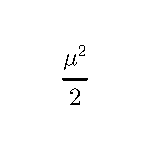
\includegraphics[width=0.5\linewidth]{../Figures/extrafont-embed} 

}

\caption{The axis title using the \texttt{extrafont} package}\label{fig:unnamed-chunk-2}
\end{figure}

\begin{Shaded}
\begin{Highlighting}[]
\NormalTok{expr2 <-}\StringTok{ }\KeywordTok{expression}\NormalTok{(}\KeywordTok{bgroup}\NormalTok{(}\StringTok{"("}\NormalTok{, }\KeywordTok{frac}\NormalTok{(x }\OperatorTok{-}\StringTok{ }\NormalTok{mu, sigma), }\StringTok{")"}\NormalTok{))}
\KeywordTok{pdf}\NormalTok{(}\StringTok{"extrafont-2.pdf"}\NormalTok{, }\DataTypeTok{width =} \DecValTok{1}\NormalTok{, }\DataTypeTok{height =} \DecValTok{1}\NormalTok{)}
\KeywordTok{grid.text}\NormalTok{(expr2, }\DataTypeTok{gp =} \KeywordTok{gpar}\NormalTok{(}\DataTypeTok{fontfamily =} \StringTok{"CM Roman"}\NormalTok{))}
\KeywordTok{dev.off}\NormalTok{()}
\KeywordTok{embed_fonts}\NormalTok{(}\StringTok{"extrafont-2.pdf"}\NormalTok{, }\DataTypeTok{outfile =} \StringTok{"extrafont-2-embed.pdf"}\NormalTok{)}
\end{Highlighting}
\end{Shaded}

\begin{figure}

{\centering 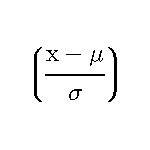
\includegraphics[width=0.5\linewidth]{../Figures/extrafont-2-embed} 

}

\caption{Another equation using the \texttt{extrafont} package}\label{fig:bracExampleExtra}
\end{figure}

In the case of figure \ref{fig:bracExampleExtra}, note how
\texttt{extrafont} has once again used the correct font for the greek
symbols, but does not quite replicate the rest of the result from
\LaTeX{}, as in \ref{bracExample}.

\begin{figure}\label{bracExample}
\centering
$\left(\dfrac{x - \mu}{\sigma}\right)$
\caption{A \LaTeX{} equation with brackets}
\end{figure}

\begin{Shaded}
\begin{Highlighting}[]
\CommentTok{# Using the 'tikzDevice' package}
\KeywordTok{library}\NormalTok{(tikzDevice)}
\KeywordTok{options}\NormalTok{(}\DataTypeTok{tikzDocumentDeclaration =} \StringTok{"}\CharTok{\textbackslash{}\textbackslash{}}\StringTok{documentclass[12pt]\{article\}"}\NormalTok{)}
\NormalTok{packages <-}\StringTok{ }\KeywordTok{c}\NormalTok{(}\KeywordTok{getOption}\NormalTok{(}\StringTok{"tikzLatexPackages"}\NormalTok{),}
              \StringTok{"}\CharTok{\textbackslash{}\textbackslash{}}\StringTok{usepackage\{amsmath\}}\CharTok{\textbackslash{}n}\StringTok{"}\NormalTok{)}
\KeywordTok{options}\NormalTok{(}\StringTok{"tikzLatexPackages"}\NormalTok{ =}\StringTok{ }\NormalTok{packages) }

\KeywordTok{tikz}\NormalTok{(}\StringTok{"tikzDevice.tex"}\NormalTok{, }\DataTypeTok{standAlone =} \OtherTok{TRUE}\NormalTok{)}
\NormalTok{opar <-}\StringTok{ }\KeywordTok{par}\NormalTok{(}\DataTypeTok{mar =} \KeywordTok{par}\NormalTok{()}\OperatorTok{$}\NormalTok{mar }\OperatorTok{+}\StringTok{ }\KeywordTok{c}\NormalTok{(}\DecValTok{0}\NormalTok{, }\DecValTok{1}\NormalTok{, }\DecValTok{0}\NormalTok{, }\DecValTok{0}\NormalTok{))}
\KeywordTok{plot}\NormalTok{(x, y, }\DataTypeTok{xlab =} \StringTok{"$}\CharTok{\textbackslash{}\textbackslash{}}\StringTok{mu$"}\NormalTok{, }\DataTypeTok{ylab =} \StringTok{""}\NormalTok{, }\DataTypeTok{yaxt =} \StringTok{"n"}\NormalTok{, }\DataTypeTok{type =} \StringTok{"l"}\NormalTok{)}
\KeywordTok{axis}\NormalTok{(}\DecValTok{2}\NormalTok{, }\DataTypeTok{las =} \DecValTok{1}\NormalTok{)}
\KeywordTok{mtext}\NormalTok{(}\StringTok{"$}\CharTok{\textbackslash{}\textbackslash{}}\StringTok{dfrac\{}\CharTok{\textbackslash{}\textbackslash{}}\StringTok{mu^2\}\{2\}$"}\NormalTok{, }\DataTypeTok{side =} \DecValTok{2}\NormalTok{, }\DataTypeTok{line =} \DecValTok{3}\NormalTok{, }\DataTypeTok{las =} \DecValTok{1}\NormalTok{)}
\KeywordTok{dev.off}\NormalTok{()}
\end{Highlighting}
\end{Shaded}

\begin{figure}\label{tikzDevicePlot}
\centering
 
\begin{tikzpicture}[x=1pt,y=1pt,scale=0.5]
\definecolor{fillColor}{RGB}{255,255,255}
\path[use as bounding box,fill=fillColor,fill opacity=0.00] (0,0) rectangle (505.89,505.89);
\begin{scope}
\path[clip] ( 73.44, 73.44) rectangle (475.65,446.85);
\definecolor{drawColor}{RGB}{0,0,0}

\path[draw=drawColor,line width= 0.4pt,line join=round,line cap=round] ( 88.34, 87.27) --
    (181.44,130.49) --
    (274.55,202.52) --
    (367.65,303.36) --
    (460.75,433.02);
\end{scope}
\begin{scope}
\path[clip] (  0.00,  0.00) rectangle (505.89,505.89);
\definecolor{drawColor}{RGB}{0,0,0}

\path[draw=drawColor,line width= 0.4pt,line join=round,line cap=round] ( 88.34, 73.44) -- (460.75, 73.44);

\path[draw=drawColor,line width= 0.4pt,line join=round,line cap=round] ( 88.34, 73.44) -- ( 88.34, 66.24);

\path[draw=drawColor,line width= 0.4pt,line join=round,line cap=round] (181.44, 73.44) -- (181.44, 66.24);

\path[draw=drawColor,line width= 0.4pt,line join=round,line cap=round] (274.55, 73.44) -- (274.55, 66.24);

\path[draw=drawColor,line width= 0.4pt,line join=round,line cap=round] (367.65, 73.44) -- (367.65, 66.24);

\path[draw=drawColor,line width= 0.4pt,line join=round,line cap=round] (460.75, 73.44) -- (460.75, 66.24);

\node[text=drawColor,anchor=base,inner sep=0pt, outer sep=0pt, scale=  1.00] at ( 88.34, 47.52) {1};

\node[text=drawColor,anchor=base,inner sep=0pt, outer sep=0pt, scale=  1.00] at (181.44, 47.52) {2};

\node[text=drawColor,anchor=base,inner sep=0pt, outer sep=0pt, scale=  1.00] at (274.55, 47.52) {3};

\node[text=drawColor,anchor=base,inner sep=0pt, outer sep=0pt, scale=  1.00] at (367.65, 47.52) {4};

\node[text=drawColor,anchor=base,inner sep=0pt, outer sep=0pt, scale=  1.00] at (460.75, 47.52) {5};

\path[draw=drawColor,line width= 0.4pt,line join=round,line cap=round] ( 73.44, 73.44) --
    (475.65, 73.44) --
    (475.65,446.85) --
    ( 73.44,446.85) --
    ( 73.44, 73.44);
\end{scope}
\begin{scope}
\path[clip] (  0.00,  0.00) rectangle (505.89,505.89);
\definecolor{drawColor}{RGB}{0,0,0}

\node[text=drawColor,anchor=base,inner sep=0pt, outer sep=0pt, scale=  1.00] at (274.55, 18.72) {$\mu$};
\end{scope}
\begin{scope}
\path[clip] (  0.00,  0.00) rectangle (505.89,505.89);
\definecolor{drawColor}{RGB}{0,0,0}

\path[draw=drawColor,line width= 0.4pt,line join=round,line cap=round] ( 73.44,130.49) -- ( 73.44,418.61);

\path[draw=drawColor,line width= 0.4pt,line join=round,line cap=round] ( 73.44,130.49) -- ( 66.24,130.49);

\path[draw=drawColor,line width= 0.4pt,line join=round,line cap=round] ( 73.44,188.11) -- ( 66.24,188.11);

\path[draw=drawColor,line width= 0.4pt,line join=round,line cap=round] ( 73.44,245.74) -- ( 66.24,245.74);

\path[draw=drawColor,line width= 0.4pt,line join=round,line cap=round] ( 73.44,303.36) -- ( 66.24,303.36);

\path[draw=drawColor,line width= 0.4pt,line join=round,line cap=round] ( 73.44,360.99) -- ( 66.24,360.99);

\path[draw=drawColor,line width= 0.4pt,line join=round,line cap=round] ( 73.44,418.61) -- ( 66.24,418.61);

\node[text=drawColor,anchor=base east,inner sep=0pt, outer sep=0pt, scale=  1.00] at ( 59.04,126.36) {2};

\node[text=drawColor,anchor=base east,inner sep=0pt, outer sep=0pt, scale=  1.00] at ( 59.04,183.98) {4};

\node[text=drawColor,anchor=base east,inner sep=0pt, outer sep=0pt, scale=  1.00] at ( 59.04,241.61) {6};

\node[text=drawColor,anchor=base east,inner sep=0pt, outer sep=0pt, scale=  1.00] at ( 59.04,299.23) {8};

\node[text=drawColor,anchor=base east,inner sep=0pt, outer sep=0pt, scale=  1.00] at ( 59.04,356.86) {10};

\node[text=drawColor,anchor=base east,inner sep=0pt, outer sep=0pt, scale=  1.00] at ( 59.04,414.48) {12};

\node[text=drawColor,anchor=base east,inner sep=0pt, outer sep=0pt, scale=  1.00] at ( 30.24,256.01) {$\dfrac{\mu^2}{2}$};
\end{scope}
\end{tikzpicture}
 \caption{Drawing the plot with the \texttt{tikzDevice} package}
 \end{figure}

The \texttt{tikzDevice} package in R will draw the axis titles with
\TeX{} but will also use \TeX{} for all other text on the plot, like the
axis labels in figure \ref{tikzDevicePlot}. This may be appropriate if
the graphic is to be included in a \TeX{} document but not so much for
other document formats like HTML.

What we want is a middle ground - being able to harness the power of
\TeX{} and its typesetting capabilities on \emph{our} choice of text or
equation in R graphics. This is where the \texttt{dvir} package comes in
- providing a simple user interface, in the style of R \texttt{grid}
graphics, by way of the \texttt{grid.latex()} function.

\begin{Shaded}
\begin{Highlighting}[]
\KeywordTok{library}\NormalTok{(dvir)}
\NormalTok{preamble <-}\StringTok{ "}\CharTok{\textbackslash{}\textbackslash{}}\StringTok{documentclass[12pt]\{standalone\}}\CharTok{\textbackslash{}n\textbackslash{}\textbackslash{}}\StringTok{usepackage\{amsmath\}}\CharTok{\textbackslash{}n\textbackslash{}\textbackslash{}}\StringTok{begin\{document\}"}
\KeywordTok{par}\NormalTok{(}\DataTypeTok{mar =} \KeywordTok{par}\NormalTok{()}\OperatorTok{$}\NormalTok{mar }\OperatorTok{+}\StringTok{ }\KeywordTok{c}\NormalTok{(}\DecValTok{0}\NormalTok{, }\DecValTok{1}\NormalTok{, }\DecValTok{0}\NormalTok{, }\DecValTok{0}\NormalTok{))}
\KeywordTok{plot}\NormalTok{(x, y, }\DataTypeTok{xlab =} \StringTok{""}\NormalTok{, }\DataTypeTok{ylab =} \StringTok{""}\NormalTok{, }\DataTypeTok{yaxt =} \StringTok{"n"}\NormalTok{, }\DataTypeTok{type =} \StringTok{"l"}\NormalTok{)}
\KeywordTok{axis}\NormalTok{(}\DecValTok{2}\NormalTok{, }\DataTypeTok{las =} \DecValTok{1}\NormalTok{)}

\KeywordTok{grid.latex}\NormalTok{(}\StringTok{"$}\CharTok{\textbackslash{}\textbackslash{}}\StringTok{mu$"}\NormalTok{, }\DataTypeTok{x =} \FloatTok{0.545}\NormalTok{, }\DataTypeTok{y =} \FloatTok{0.07}\NormalTok{)}
\KeywordTok{grid.latex}\NormalTok{(}\StringTok{"$}\CharTok{\textbackslash{}\textbackslash{}}\StringTok{dfrac\{}\CharTok{\textbackslash{}\textbackslash{}}\StringTok{mu^2\}\{2\}$"}\NormalTok{, }\DataTypeTok{x =} \FloatTok{0.06}\NormalTok{, }\DataTypeTok{preamble =}\NormalTok{ preamble)}
\end{Highlighting}
\end{Shaded}

\begin{figure}

{\centering \includegraphics[width=0.7\linewidth]{Alexander-van-der-Voorn_dissertation_files/figure-latex/plotGridLatex-1} 

}

\caption{Changing axis titles with \texttt{grid.latex()}}\label{fig:plotGridLatex}
\end{figure}

Figure \ref{fig:plotGridLatex} recreates figure \ref{fig:expressionPlot}
with the axis titles made using \texttt{grid.latex()}.

\subsection{Where this project fits
in}\label{where-this-project-fits-in}

The \texttt{dvir} package already worked really well in a lot of cases.
There were however a number of desirable features of \TeX{} and its
extensions that had not yet been implemented by \texttt{dvir}. The power
of this package comes from ensuring it is comprehensive enough to meet a
user's entire \TeX{} needs in R graphics without having to leave R to do
annotations in \LaTeX{} itself (or other software like Adobe Photoshop
or Illustrator).

By keeping things ``in R'' users only need to learn R (and basic \TeX)
code to create their graphics and their work is in one place and easily
reproducible. It may not be realistic to \emph{completely} replicate
\TeX{} in R, however several aspects of the package were identified as
having the potential to increase its usefulness. The aspects identified
were:

\begin{itemize}
\tightlist
\item
  the speed of the package - anecdotally it took a while to generate
  graphics, especially if there were many \texttt{grid.latex()} calls
\item
  expand \texttt{dvir}'s capability of creating \Tikz{} drawings by
  adding support for linear gradient fills
\item
  adding the ability to align text from \texttt{grid.latex()} to a
  baseline - the natural line on which characters sit
\end{itemize}

\newpage{}

\section{Background}\label{background}

\subsection{\texorpdfstring{\TeX{}}{}}\label{section}

\TeX{} is a program to format and typeset text, and includes some basic
macros to do this. \LaTeX{} is a higher-level implementation that sits
on top of \TeX{}, basically consisting of a lot more macros, creating a
much more user-friendly interface to \TeX{}. For example, \LaTeX{}
allows one to create a document with numbered sections, title pages and
bibliographies without having to write complicated \TeX{} macros
oneself.

\subsection{DVI}\label{dvi}

A \TeX{} or \LaTeX{} file is just plain text so there needs to be a step
to translate this plain text to what you will see on a formatted
document on a screen or page. \TeX{} ``engine'' like \texttt{pdflatex}
normally processes \TeX{} to PDF but it can also produce a DVI (DeVice
Independent) file. A DVI file is a binary file describing the layout of
the document. For example, the height of the page, what characters to
display and where, and the fonts to be used. DVI provides a format that
can be read into R so that we can draw the \TeX{} layout in R. This is
what the \texttt{dvir} package does.

\subsection{\texorpdfstring{The (pre-existing) \texttt{dvir}
package}{The (pre-existing) dvir package}}\label{dvirDesc}

In a simplified form, \texttt{dvir} works by providing a high level
function, \texttt{grid.latex()}, to call with the \TeX{} code of the
expression or text to be displayed. In this instance, the preamble is
changed only because the axis title uses \texttt{\textbackslash{}dfrac}
so the \texttt{amsmath} package needs to be specified in the preamble.

\begin{Shaded}
\begin{Highlighting}[]
\KeywordTok{library}\NormalTok{(dvir)}
\NormalTok{texCode <-}\StringTok{ "$}\CharTok{\textbackslash{}\textbackslash{}}\StringTok{dfrac\{}\CharTok{\textbackslash{}\textbackslash{}}\StringTok{mu^2\}\{2\}$"}
\NormalTok{newPreamble <-}\StringTok{ }
\StringTok{  "}\CharTok{\textbackslash{}\textbackslash{}}\StringTok{documentclass[12pt]\{standalone\}}\CharTok{\textbackslash{}n\textbackslash{}\textbackslash{}}\StringTok{usepackage\{amsmath\}}\CharTok{\textbackslash{}n\textbackslash{}\textbackslash{}}\StringTok{begin\{document\}"}
\KeywordTok{grid.latex}\NormalTok{(texCode, }\DataTypeTok{preamble =}\NormalTok{ newPreamble)}
\end{Highlighting}
\end{Shaded}

\begin{figure}

{\centering \includegraphics[width=0.7\linewidth]{Alexander-van-der-Voorn_dissertation_files/figure-latex/unnamed-chunk-6-1} 

}

\caption{Using the \texttt{dvir} function \texttt{grid.latex()}}\label{fig:unnamed-chunk-6}
\end{figure}

The following steps are taken when \texttt{grid.latex()} runs:

\begin{enumerate}
  \item A \TeX{} document is created with the expression and a changeable default preamble and postamble.
\end{enumerate}

\begin{Shaded}
\begin{Highlighting}[]
\NormalTok{postamble <-}\StringTok{ }\KeywordTok{paste0}\NormalTok{(}\StringTok{"}\CharTok{\textbackslash{}\textbackslash{}}\StringTok{end\{document\}"}\NormalTok{)}
\KeywordTok{cat}\NormalTok{(}\KeywordTok{paste}\NormalTok{(newPreamble,}
\NormalTok{          texCode,}
\NormalTok{          postamble,}
          \DataTypeTok{sep =} \StringTok{"}\CharTok{\textbackslash{}n}\StringTok{"}\NormalTok{))}
\end{Highlighting}
\end{Shaded}

\begin{itemize}[noitemsep]
  \item[] \begin{verbatim}\documentclass[12pt]{standalone}\end{verbatim}
  \item[] \begin{verbatim}\usepackage{amsmath}\end{verbatim}
  \item[] \begin{verbatim}\begin{document}\end{verbatim} 
  \item[] \begin{verbatim}$\dfrac{\mu^2}{2}$\end{verbatim}
  \item[] \begin{verbatim}\end{document}\end{verbatim}
\end{itemize}

\begin{enumerate}
  \setcounter{enumi}{1}
  \item This TeX document is then processed using the local \TeX{} installation to create a DVI (DeVice Independent) file.
  \item The DVI file is read into R. As DVI files are binary they are not easily readable by humans but the \texttt{dvir} function \texttt{readDVI()} translates the DVI file into readable text. This is an extract of a DVI file after using \texttt{readDVI()}, stating the definition of a font and then "setting", that is, printing, a character "2".
\end{enumerate}

\begin{itemize}[noitemsep]
  \item[] \begin{verbatim}fnt_def_1    fontnum=15, checksum=2088458503, scale=524288,\end{verbatim}
  \item[] \begin{verbatim}             design=524288, fontname=cmr8\end{verbatim}
  \item[] \begin{verbatim}set_char_50  '2'\end{verbatim}
\end{itemize}

\begin{enumerate}
  \setcounter{enumi}{3}
  \item Three "sweeps" of the DVI file are completed to extract necessary information about what to display in R (and where and how to display it):
  \begin{itemize}
    \item Font sweep: Gather the names of all fonts used in the DVI file and locate the relevant font files on the local machine. The font information is stored in a R list as well as a \texttt{fontconfig} file.
    \item Metric sweep: To determine the overall bounding box (size) of the expression to display. This bounding box is used to create a \texttt{grid} viewport which can encompass the entire \TeX{} passed to \texttt{grid.latex()} expression using the native DVI coordinates.
    \item Grid sweep: Convert all text and symbols into \textit{grobs} (grid graphical objects) 
  \end{itemize}
  \item These grobs are then displayed in the R graphics device as per the \texttt{grid} package.
\end{enumerate}

\newpage{}

\section{Code speed (part 1) - removing redundant font
sweeps}\label{code-speed-part-1---removing-redundant-font-sweeps}

In the introduction of this report the case for the \texttt{dvir}
package was motivated with a simple example of a mathematical equation.
\texttt{dvir} can be used on a larger scale too.

\begin{Shaded}
\begin{Highlighting}[]
\KeywordTok{grid.latex}\NormalTok{(}\StringTok{"}\CharTok{\textbackslash{}\textbackslash{}}\StringTok{dots"}\NormalTok{, }\DataTypeTok{x =} \FloatTok{0.44}\NormalTok{, }\DataTypeTok{y =} \FloatTok{-0.1}\NormalTok{, }\DataTypeTok{default.units=}\StringTok{"native"}\NormalTok{)}
\KeywordTok{grid.latex}\NormalTok{(}\StringTok{"$Y_* =$"}\NormalTok{, }\DataTypeTok{x =} \FloatTok{0.5}\NormalTok{, }\DataTypeTok{y =} \FloatTok{1.1}\NormalTok{, }\DataTypeTok{default.units=}\StringTok{"native"}\NormalTok{)}
\KeywordTok{grid.latex}\NormalTok{(}\StringTok{"$a_1$"}\NormalTok{, xpos[}\DecValTok{1}\NormalTok{], }\DataTypeTok{y =} \FloatTok{-0.1}\NormalTok{, }\DataTypeTok{default.units=}\StringTok{"native"}\NormalTok{)}
\KeywordTok{grid.latex}\NormalTok{(}\StringTok{"$a_2$"}\NormalTok{, xpos[}\DecValTok{2}\NormalTok{], }\DataTypeTok{y =} \FloatTok{-0.1}\NormalTok{, }\DataTypeTok{default.units=}\StringTok{"native"}\NormalTok{)}
\KeywordTok{grid.latex}\NormalTok{(}\StringTok{"$a_\{L_A\}$"}\NormalTok{, xpos[}\DecValTok{3}\NormalTok{], }\DataTypeTok{y =} \FloatTok{-0.1}\NormalTok{, }\DataTypeTok{default.units=}\StringTok{"native"}\NormalTok{)}
\KeywordTok{grid.latex}\NormalTok{(}\StringTok{"$Y_\{}\CharTok{\textbackslash{}\textbackslash{}}\StringTok{pi\} | Y_\{}\CharTok{\textbackslash{}\textbackslash{}}\StringTok{pi\} }\CharTok{\textbackslash{}\textbackslash{}}\StringTok{notin }\CharTok{\textbackslash{}\textbackslash{}}\StringTok{cal\{A\}$"}\NormalTok{, }
           \DataTypeTok{x =}\NormalTok{ xpos[}\DecValTok{4}\NormalTok{], }\DataTypeTok{y =} \FloatTok{-0.1}\NormalTok{, }\DataTypeTok{default.units=}\StringTok{"native"}\NormalTok{)}
\KeywordTok{grid.latex}\NormalTok{(}\StringTok{"$}\CharTok{\textbackslash{}\textbackslash{}}\StringTok{omega_1$"}\NormalTok{, }\DataTypeTok{x =} \FloatTok{0.18}\NormalTok{, }\DataTypeTok{y =} \FloatTok{0.50}\NormalTok{, }\DataTypeTok{default.units=}\StringTok{"native"}\NormalTok{)}
\KeywordTok{grid.latex}\NormalTok{(}\StringTok{"$}\CharTok{\textbackslash{}\textbackslash{}}\StringTok{omega_2$"}\NormalTok{, }\DataTypeTok{x =} \FloatTok{0.32}\NormalTok{, }\DataTypeTok{y =} \FloatTok{0.50}\NormalTok{, }\DataTypeTok{default.units=}\StringTok{"native"}\NormalTok{)}
\KeywordTok{grid.latex}\NormalTok{(}\StringTok{"$}\CharTok{\textbackslash{}\textbackslash{}}\StringTok{dots$"}\NormalTok{, }\DataTypeTok{x =} \FloatTok{0.44}\NormalTok{, }\DataTypeTok{y =} \FloatTok{0.50}\NormalTok{, }\DataTypeTok{default.units=}\StringTok{"native"}\NormalTok{)}
\KeywordTok{grid.latex}\NormalTok{(}\StringTok{"$}\CharTok{\textbackslash{}\textbackslash{}}\StringTok{omega_\{L_A\}$"}\NormalTok{,  }\DataTypeTok{x =} \FloatTok{0.54}\NormalTok{, }\DataTypeTok{y =} \FloatTok{0.50}\NormalTok{, }\DataTypeTok{default.units=}\StringTok{"native"}\NormalTok{)}
\KeywordTok{grid.latex}\NormalTok{(}\StringTok{"$1 - }\CharTok{\textbackslash{}\textbackslash{}}\StringTok{sum_\{s=1\}^\{L_A\}}\CharTok{\textbackslash{}\textbackslash{}}\StringTok{omega_s$"}\NormalTok{, }\DataTypeTok{x =} \FloatTok{0.95}\NormalTok{, }\DataTypeTok{y =} \FloatTok{0.50}\NormalTok{, }\DataTypeTok{default.units=}\StringTok{"native"}\NormalTok{)}
\end{Highlighting}
\end{Shaded}

\begin{figure}

{\centering \includegraphics[width=0.7\linewidth]{Alexander-van-der-Voorn_dissertation_files/figure-latex/yeeExample-1} 

}

\caption{Using nine \texttt{grid.latex()} calls with base R graphics.}\label{fig:yeeExample}
\end{figure}

The example in figure \ref{fig:yeeExample} was created by a University
of Auckland lecturer using the \texttt{dvir} package to help write an
assignment.

One of the first things investigated in the package was the speed of
running the code. Anecdotally, generating any R graphic with non-trivial
\TeX{}, like that in figure \ref{fig:yeeExample}, took a long time so it
was desirable to speed it up.

To look into this the first task was to profile the existing code to let
us see where in the package time was being spent. This was in
\texttt{dvir} version 0.2-1. The profiling results were visualised with
\texttt{profvis::profvis()}.

\begin{figure}

{\centering 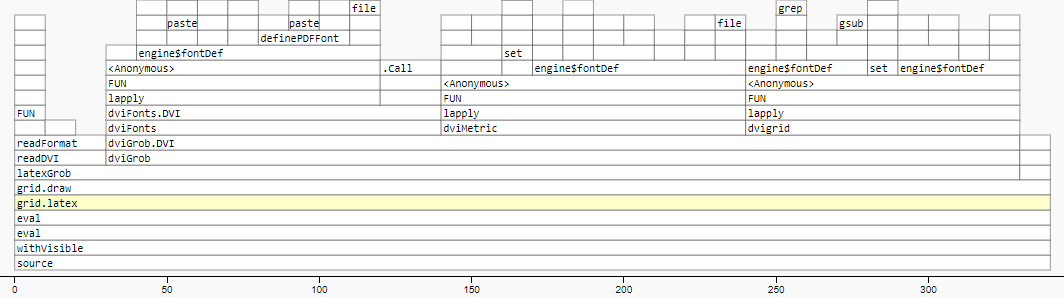
\includegraphics[width=1\linewidth]{../Figures/profilingSimpleProfvis_0.2-1} 

}

\caption{Screenshot of \texttt{profvis::profvis()} output for the simple example in \texttt{dvir} version 0.2-1.}\label{fig:prof1}
\end{figure}

We can see the function call stack in figure \ref{fig:prof1}. At the
bottom is the call to \texttt{grid.latex()}, which immediately calls
\texttt{grid.draw()} which in turn calls \texttt{latexGrob()}. This
calls \texttt{readDVI()} for about the first 20ms, then
\texttt{dviGrob()} for the remaining time to the end of the original
\texttt{grid.latex()} function call, and so on up the function call
stack.

\begin{figure}

{\centering 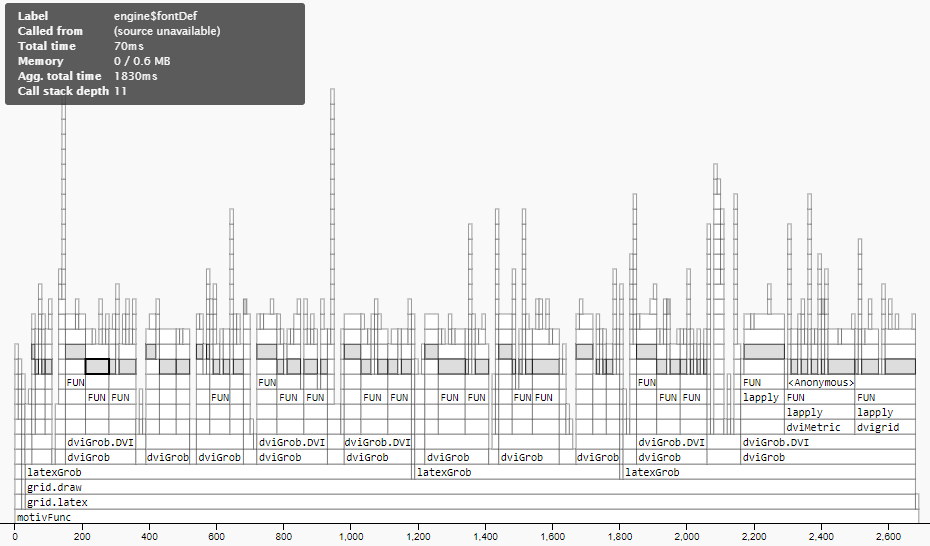
\includegraphics[width=1\linewidth]{../Figures/profilingYeeProfvis_0.2-1_highlight} 

}

\caption{Screenshot of \texttt{profvis::profvis()} output for the code creating the example at the start of this section, highlighting the time spent in \texttt{engine\$fontDef}.}\label{fig:prof2}
\end{figure}

The \texttt{profvis::profvis()} output for our more complicated example,
in figure \ref{fig:prof2} reveals most of the time to create the figure
is in \texttt{grid.latex()}. Note that the code to draw the arrows and
the ``(a)'' in this example is so quick it occupies the very skinny call
stack on the far left of the graph. \texttt{grid.latex()} and its
subsequent function calls, on the other hand, take up most of the time
required to produce the example.

In figure \ref{fig:prof2} some blocks in the call stack have been
highlighted - these are related to the \texttt{engine\$fontDef}
operation occuring. This is a part of the ``font sweep'', as was
described in the introduction to \texttt{dvir} in section
\ref{dvirDesc}.

In the top left corner of figure \ref{fig:prof2} we are told the
aggregate time spent with \texttt{engine\$fontDef} is 1830ms. Compared
to the total time of this run (a total of about 2700ms), \texttt{dvir}
is spending a \emph{lot} of time doing these font sweeps.

What was interesting though was that after the actual font sweep the
following sweeps for the metric and grid information \emph{also} called
\texttt{engine\$fontDef}. As the point of the font sweep is that it
finds all the font information to be used later on the following metric
and grid sweeps should not need to ``re-sweep'' for the fonts.

\begin{figure}

{\centering 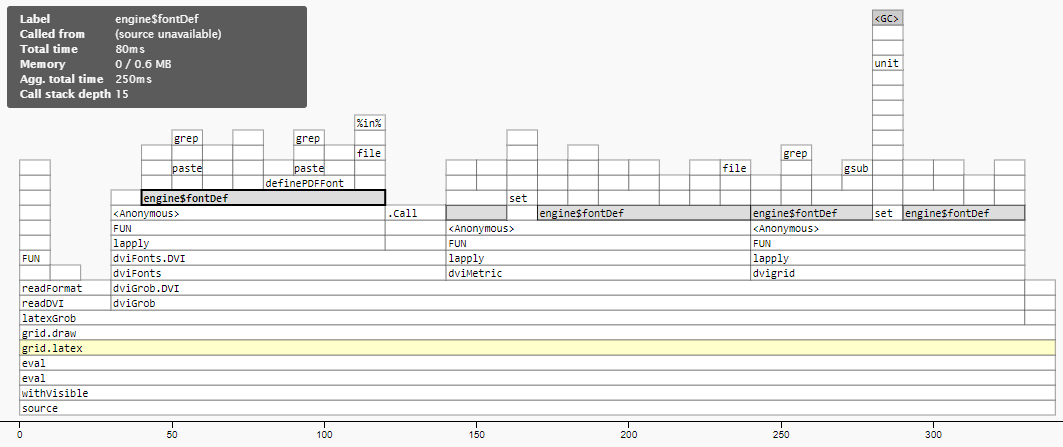
\includegraphics[width=1\linewidth]{../Figures/profilingSimpleProfvis_0.2-1_highlight} 

}

\caption{Screenshot of \texttt{profvis::profvis()} output for the simple example in \texttt{dvir} version 0.2-1, highlighting \texttt{engine\$fontDef}.}\label{fig:prof3}
\end{figure}

The effect of this is very obvious in figure \ref{fig:prof3} which is
the same as figure \ref{fig:prof1} but highlights the time spent in
\texttt{engine\$fontDef}. The wrappers for the font, metric and grid
sweeps are \texttt{dviFonts()}, \texttt{dviMetric()} and
\texttt{dvigrid()} respectively (sixth call from the bottom of the
stack). Here we can see nearly all of the time spent in the metric and
grid sweeps are actually redoing the font sweep.

The change to be made was simply stopping the metric and grid sweeps
from doing the font sweep again.

The font sweep looks in the DVI file for op codes 243 to 246. These are
the op codes for font definitions and define the name of a font and give
it an identifier to reference in the DVI file when it wants to use that
font to display a character.

The following code is taken from the the \texttt{dvir} package, showing
where the metric and grid sweeps also redid the font sweep.
\texttt{op\_font\_def} is a function which takes the font definition in
the DVI file related to that instance of the op code and searches for
and records the font information.

\begin{Shaded}
\begin{Highlighting}[]
\NormalTok{metric_info_}\DecValTok{243}\NormalTok{ <-}\StringTok{ }\NormalTok{op_font_def}
\NormalTok{grid_op_}\DecValTok{243}\NormalTok{ <-}\StringTok{ }\NormalTok{op_font_def}
\end{Highlighting}
\end{Shaded}

The following code shows what the code was changed to in \texttt{dvir}
version 0.2-2. \texttt{op\_ignore} is an empty function, so when the
metric or grid sweeps comes across that op code, they now do nothing.

\begin{Shaded}
\begin{Highlighting}[]
\NormalTok{metric_info_}\DecValTok{243}\NormalTok{ <-}\StringTok{ }\NormalTok{op_ignore}
\NormalTok{grid_op_}\DecValTok{243}\NormalTok{ <-}\StringTok{ }\NormalTok{op_ignore}
\end{Highlighting}
\end{Shaded}

Unfortunately these changes by themself caused an error when running
\texttt{grid.latex()}. This is because one task undertaken before the
font sweep is to reset or overwrite the global fonts list (which the
font sweep then writes to). The metric and grid sweeps were also doing
this even though it was only intended for it to be done by the font
sweep. This meant after the font sweep was completed it was overwritten
by the metric and grid sweeps and so when \texttt{dvir} tried to draw
the characters there was no font information to refer to.

The resetting of the global fonts list was initiated when the sweeps
passed op code 247 in the DVI file, which is the preamble at the start
of every DVI file. Setting the metric and grid sweeps to do nothing when
they pass the preamble of the DVI file, again by way of
\texttt{op\_ignore}, solved this problem as the global fonts list
created by the font sweep is now not overwritten.

\begin{Shaded}
\begin{Highlighting}[]
\NormalTok{metric_info_}\DecValTok{247}\NormalTok{ <-}\StringTok{ }\NormalTok{op_ignore}
\NormalTok{grid_op_}\DecValTok{247}\NormalTok{ <-}\StringTok{ }\NormalTok{op_ignore}
\end{Highlighting}
\end{Shaded}

To quantify the impact this has on code speed the time to run the
examples 20 times was recorded, after an initial run to compile the
package after it was loaded. The average of these 20 runs was then
calculated.

\begin{figure}

{\centering \includegraphics[width=0.7\linewidth]{Alexander-van-der-Voorn_dissertation_files/figure-latex/speedUp1Simple-1} 

}

\caption{The average time spent in the \texttt{grid.latex()} function, metric sweep and grid sweep before and after these changes, for each of the 20 runs of the simple example.}\label{fig:speedUp1Simple}
\end{figure}

For the simple example the time spent in the metric and grid sweeps have
decreased by 76\% and 83\% respectively. The speed of the overall
\texttt{grid.latex()} call has decreased by 30\%.

\begin{figure}

{\centering \includegraphics[width=0.7\linewidth]{Alexander-van-der-Voorn_dissertation_files/figure-latex/speedUp1Yee-1} 

}

\caption{The average time spent in the \texttt{grid.latex()} function, metric sweep and grid sweep before and after these changes, for each of the 20 runs of the complicated example.}\label{fig:speedUp1Yee}
\end{figure}

Similarly for the more complicated example in figure
\ref{fig:speedUp1Yee} the metric and grid sweeps have decreased by 83\%
and 89\% respectively, with \texttt{grid.latex()} overall taking 47\%
less time.

\newpage{}

\section{Code speed (part 2) - font
caching}\label{code-speed-part-2---font-caching}

In the previous section, the speed of \texttt{dvir} was increased by
stopping it doing something ``silly''. The profiling results from the
previous section demonstrate how much time \texttt{grid.latex()} spends
dealing with fonts so this section is about making \texttt{dvir}
``smarter'' by caching the information it gathers about fonts between
\texttt{grid.latex()} calls.

For example, creating figure \ref{fig:yeeExample} requires three
\texttt{grid.latex()} calls for the same symbol \(\omega\). Each time,
the following font definition appears in the DVI file for
\texttt{grid.latex()} to search for during its font sweep.

\begin{verbatim}
fnt_def_1    fontnum=17, checksum=-1209964637, scale=786432, design=786432,
             fontname=cmmi12
\end{verbatim}

In fact, the example's 11 \texttt{grid.latex()} calls define fonts 29
times in total, for eight unique fonts.

Caching fonts requires several steps:

\begin{itemize}
  \item During the font sweep, search all font definitions as per usual.
  \item For each font definition, check if the font has been cached already.
  \begin{itemize}
    \item If yes, do nothing. Refer to the existing font information in the cache when the needs to be used
    \item If no, search for and store the font information as per usual.
  \end{itemize}
\end{itemize}

The font information is stored in R as a list. Every time
\texttt{grid.latex()} processed a ``preamble'' op code in a DVI file,
that is, every time \texttt{grid.latex()} was called, the font list was
initialised as an empty list in the \texttt{dvir} namespace with
\texttt{dvir::set("fonts",\ vector("list",\ 255))}. To stop this
initialisation happening by default, the following code was put in its
place.

\begin{verbatim}
if (dvir::get("initFonts") || is.null(dvir::get("fonts"))) dvir::set("fonts", vector("list", 255))
\end{verbatim}

Note in this new statement the logical variable \texttt{initFonts},
stored in the \texttt{dvir} namespace. This lets a user choose whether
to intialise the font cache on a \texttt{grid.latex()} call. If
\texttt{initFonts} is \texttt{FALSE} or the font list does not exist,
for example after the package is loaded, the font list is initialised.
Otherwise, the existing font cache remains. \texttt{initFonts} was added
as an argument to \texttt{grid.latex()} with its default value being
equal to the global option \texttt{dvir.initFonts}.

In a DVI file, each font definition gives the font a identification
number, for example \texttt{fontnum=17}. In all the DVI files examined
as part of this project, this font identification number is the same
when that particular font is used again in another \texttt{grid.latex()}
call. This number is used as the index of the fonts list where its
information is stored.

When the font sweep passes a font definition in the DVI file it checks
first whether the index of the font list matching the font number of the
new font contains any existing font information:

\begin{itemize}
  \item If no, then the font information is written to the font list as usual.
  \item If yes, then it checks if the existing font information is the same as the font information in the DVI file. 
  \begin{itemize}
    \item If yes, do nothing. 
    \item If no, overwrite the font with the new font information.
  \end{itemize}
\end{itemize}

The result of this is that across multiple \texttt{grid.latex()} calls
requiring the same fonts, any future uses of that font are much faster
after the font has been used once. Importantly it also has a ``fail
safe'' where if there happens to be a case where the font number was
used with a different font in a previous \texttt{grid.latex()} call, the
font cache is overwritten with the new font so the correct font will be
used.

The updated font list is stored in the \texttt{dvir} environment to be
retrieved the next \texttt{grid.latex()} finds a font definition during
a font sweep.

The only weakness of this process is if in a \emph{single} DVI file
different fonts are defined with the same font number. In this case the
second font will be stored in the font cache in that index and so will
be used in place of the first font. No instances of this occurring were
discovered during this project.

To examine the effect of these changes on code speed we performed
profiling as was detailed in the previous section.

\begin{figure}

{\centering \includegraphics[width=0.7\linewidth]{Alexander-van-der-Voorn_dissertation_files/figure-latex/speedUp2Simple-1} 

}

\caption{The average time spent in the \texttt{grid.latex()} function and font sweep for each of the 20 runs of the simple example.}\label{fig:speedUp2Simple}
\end{figure}

For the simple example the time for the font sweep has reduced by 71\%,
with \texttt{grid.latex()} overall taking 45\% less time.

\begin{figure}

{\centering \includegraphics[width=0.7\linewidth]{Alexander-van-der-Voorn_dissertation_files/figure-latex/speedUp2Yee-1} 

}

\caption{The average time spent in the \texttt{grid.latex()} function and font sweep for each of the 20 runs of the complicated example}\label{fig:speedUp2Yee}
\end{figure}

Similar results can be seen in for the example in figure
\ref{fig:yeeExample} - a 76\% and 46\% decrease in the font sweep and
\texttt{grid.latex()} respectively.

\subsection{Profiling environment
specifications}\label{profiling-environment-specifications}

The exact results obtained in this and the previous section are specific
to the computing environment used. Specific details are provided below.
The sampling nature of profiling (intermittent recording of the call
stack) will give different results every time it is done.

The profiling results are dependent on the computer setup used and could
change depending on the exact computing environment in which the
\texttt{dvir} package is used.

The profiling results in this report, in this and the previous section,
were calculated with the following setup:

\begin{itemize}
\tightlist
\item
  A virtual machine via Oracle VM Virtualbox
\item
  Virtual machine running Ubuntu 18.04.5 LTS
\item
  R version 3.4.4
\item
  \texttt{dvir} package versions as described with the profiling results
\end{itemize}

\newpage{}

\section{Linear gradient fills}\label{linear-gradient-fills}

\subsection{\texorpdfstring{\Tikz{} and
\texttt{dvir}}{ and dvir}}\label{and-dvir}

\Tikz{} (Tantau 2021) is a \TeX{} package that allows drawing of
pictures and diagrams in \TeX{} documents.

\begin{spacing}{1}
\begin{verbatim}
\begin{tikzpicture}
\path (0, 1) node[circle,fill=red!40,draw,thick] (x) {$\mu$}
      (3, 0) node[circle,fill=blue!40,draw,thick] (y) {$\dfrac{\mu^2}{2}$};
\draw[->] (x) .. controls (1, 0.5) and (2, 0.5).. (y);
\end{tikzpicture}
\end{verbatim}
\end{spacing}

\begin{figure}\label{tikzRaw}
\centering
\begin{tikzpicture}
\path (0, 1) node[circle,fill=red!40,draw,thick] (x) {$\mu$} 
      (3, 0) node[circle,fill=blue!40,draw,thick] (y) {$\dfrac{\mu^2}{2}$};
\draw[->] (x) .. controls (1, 0.5) and (2, 0.5).. (y);
\end{tikzpicture}
\caption{A picture made with \Tikz{}}
\end{figure}

The original DVI specification only needed to account for text,
typesetting and the most basic of rectangles and so was not designed
with drawing and graphics in mind. The type of instruction in the DVI
file are labelled with an ``op code''. Each op code described a type of
instruction like defining fonts, setting characters to display and
vertical and horizontal cursor movements. There were four op codes
however, called \emph{DVI specials}, that can contain almost any form of
instruction or values needed, such as text colour, to create a document
based on the DVI file, such as Postscript or PDF.

The \Tikz{} package uses these DVI specials to describe shapes, drawings
and colours in PGF (portable graphics format) which can be translated to
instructions for other viewing formats, like Postscript, PDF or SVG. How
the instructions are translated is controlled by a \Tikz{} driver. The
\texttt{dvir} package (Murrell 2020a) includes its own \Tikz{} driver to
translate the drawing instructions into a form useful to draw the things
with R grid graphics {[}reference Paul dvir \Tikz{} report{]}.

Some \Tikz{} features were not implemented though, notably the ability
to have fill colours of shapes as linear or radial gradients or
patterns. The primary reason for this is that R did not support these
types of fills but the latest R release in May 2021, version 4.1.0,
provides support for these fills in the \texttt{grid} package (Murrell
2020b), on which \texttt{dvir} is built.

\begin{Shaded}
\begin{Highlighting}[]
\NormalTok{tikzCode <-}\StringTok{ }\KeywordTok{paste}\NormalTok{(}\StringTok{"}\CharTok{\textbackslash{}\textbackslash{}}\StringTok{path (0, 1) node[circle,fill=red!40,draw,thick] (x) \{$}\CharTok{\textbackslash{}\textbackslash{}}\StringTok{mu$\}"}\NormalTok{,}
                  \StringTok{"      (3, 0) node[circle,fill=blue!40,draw,thick] (y) \{$}\CharTok{\textbackslash{}\textbackslash{}}\StringTok{dfrac\{}\CharTok{\textbackslash{}\textbackslash{}}\StringTok{mu^2\}\{2\}$\};"}\NormalTok{,}
                  \StringTok{"}\CharTok{\textbackslash{}\textbackslash{}}\StringTok{draw[->] (x) .. controls (1, 0.5) and (2, 0.5).. (y);"}\NormalTok{,}
                  \DataTypeTok{sep =} \StringTok{"}\CharTok{\textbackslash{}n}\StringTok{"}\NormalTok{)}
\NormalTok{tikzPreamble <-}\StringTok{ }\KeywordTok{gsub}\NormalTok{(}\StringTok{"}\CharTok{\textbackslash{}\textbackslash{}\textbackslash{}\textbackslash{}}\StringTok{usepackage}\CharTok{\textbackslash{}\textbackslash{}}\StringTok{\{tikz\}"}\NormalTok{, }
                     \StringTok{"}\CharTok{\textbackslash{}\textbackslash{}\textbackslash{}\textbackslash{}}\StringTok{usepackage\{tikz\}}\CharTok{\textbackslash{}n\textbackslash{}\textbackslash{}\textbackslash{}\textbackslash{}}\StringTok{usepackage\{amsmath\}"}\NormalTok{, }
                     \KeywordTok{tikzpicturePreamble}\NormalTok{())}
\KeywordTok{grid.tikzpicture}\NormalTok{(tikzCode, }\DataTypeTok{preamble =}\NormalTok{ tikzPreamble)}
\end{Highlighting}
\end{Shaded}

\begin{figure}

{\centering \includegraphics[width=1\linewidth]{Alexander-van-der-Voorn_dissertation_files/figure-latex/gridTikz-1} 

}

\caption{Using \texttt{grid.tikzpicture()} to make the diagram from earlier}\label{fig:gridTikz}
\end{figure}

The use of \texttt{grid.tikzpicture()} is demonstrated in figure
\ref{fig:gridTikz}, recreating the diagram from figure \ref{tikzRaw}.
The alteration to the preamble once again only necessary due to the use
of \texttt{\textbackslash{}dfrac} from the \texttt{amsmath} package.

\begin{itemize}
\tightlist
\item
  {[}\textbf{Example:} Make same \Tikz{} example as above in R with dvir
  (obviously fill will be blank){]}
\end{itemize}

As it is, the \Tikz{} driver simply ignores any gradient or pattern fill
information when creating the DVI file for \texttt{dvir}.

\begin{itemize}
\tightlist
\item
  {[}\textbf{Example:} Use \texttt{grid.tikzpicture()} for picture with
  gradient fill in text, but resulting R graphic does not have fill{]}
\end{itemize}

\subsection{\texorpdfstring{Implementing \Tikz{} linear gradient fills
in
\texttt{dvir}\label{tikzWorkflow}}{Implementing  linear gradient fills in dvir}}\label{implementing-linear-gradient-fills-in-dvir}

The following steps are required to implement these \Tikz{} fills in
\texttt{dvir}:

\begin{enumerate}
\def\labelenumi{\arabic{enumi}.}
\item
  Add the fill information (like the gradient colours and their
  locations) to the DVI file created by \texttt{dvir}
\item
  Store this fill information during a parse by \texttt{dvir} to read
  the DVI file
\item
  Add the fill information when drawing the shape in R
\end{enumerate}

To tackle step 1, we need to update the \texttt{dvir} \Tikz{} driver
file to include information about the gradient and pattern fills. As the
\texttt{dvir} \Tikz{} driver file is based on the SVG \Tikz{} driver
file, the SVG support for \Tikz{} fills was used as a base to edit to
make it specific to \texttt{dvir}.

The information we require for the gradient fills from \Tikz{} via the
DVI file is as per the arguments for the
\texttt{grid::linearGradient(...)}, which is used as an argument to
\texttt{grid::gpar(fill\ =\ linearGradient(...))}, which itself is an
argument to a \texttt{grid} drawing function, for example
\texttt{grid::grid.rect(...,\ gp\ =\ gpar(fill\ =\ linearGradient(...)))}.
The most important parts of defining a linear gradient fill is the
colours and stops of the gradient fill. The stops of a gradient fill are
the locations along the length of a gradient fill where the specified
colours are. In between the stops, the gradient between stop colours
either side occurs.

The \texttt{colours} and \texttt{stops} arguments of
\texttt{linearGradient()} are simply vectors of colours (a character
vector of colour names of hexadecimal RGB values) and locations of those
colours as a proportion of the distance between the start and end points
of the gradient respectively. This obviously guides us as to what
information we need to get from \Tikz{} in the DVI file so we can pass
it to \texttt{dvir}.

Let us consider a simple example, a rectangle with an orange to green
linear gradient fill:

\begin{figure}
\centering
\begin{tikzpicture}
\filldraw [draw=black, left color=orange, right color=green] (0,0) rectangle (4,2);
\end{tikzpicture}
\end{figure}

The following is an extract of the DVI file when the rectangle above is
generated using the SVG DVI driver included with the common \TeX{}
distributions, \texttt{pgfsys-dvisvgm.def}. It has been edited slightly
for readability by adding line breaks and removing a line break
``character'', \texttt{\{?nl\}}.

\texttt{\{\ dviGradientOutput,\ eval=FALSE\}\ xxx1\ \ \ \ \ \ \ \ \ k=67\ \ \ \ \ \ \ \ \ \ \ \ \ \ x=dvisvgm:raw\ \textless{}g\ transform="matrix(1,0,0,1,56.90549,28.45274)"\textgreater{}\ \ xxx1\ \ \ \ \ \ \ \ \ k=67\ \ \ \ \ \ \ \ \ \ \ \ \ \ x=dvisvgm:raw\ \textless{}g\ transform="matrix(2.26802,0,0,1.134,0.0,0.0)"\textgreater{}\ xxx1\ \ \ \ \ \ \ \ \ k=66\ \ \ \ \ \ \ \ \ \ \ \ \ \ x=dvisvgm:raw\ \textless{}g\ transform="matrix(0.0,1.0,-1.0,0.0,0.0,0.0)"\textgreater{}\ xxx4\ \ \ \ \ \ \ \ \ k=425\ \ \ \ \ \ \ \ \ \ \ \ \ \ x=dvisvgm:raw\ \ \textless{}linearGradient\ id="pgfsh2"\ gradientTransform="rotate(90)"\textgreater{}\ \ \ \ \ \ \ \ \ \ \ \ \ \ \ \ \ \ \ \ \ \ \ \ \ \ \ \ \ \ \textless{}stop\ offset="\ 0.0"\ stop-color="\ rgb(0.0\%,100.0\%,0.0\%)\ "/\textgreater{}\ \ \ \ \ \ \ \ \ \ \ \ \ \ \ \ \ \ \ \ \ \ \ \ \ \ \ \ \ \ \textless{}stop\ offset="\ 0.25"\ stop-color="\ rgb(0.0\%,100.0\%,0.0\%)\ "/\textgreater{}\ \ \ \ \ \ \ \ \ \ \ \ \ \ \ \ \ \ \ \ \ \ \ \ \ \ \ \ \ \textless{}stop\ offset="\ 0.5"\ stop-color="\ rgb(50.0\%,75.0\%,0.0\%)\ "/\textgreater{}\ \ \ \ \ \ \ \ \ \ \ \ \ \ \ \ \ \ \ \ \ \ \ \ \ \ \ \ \ \textless{}stop\ offset="\ 0.75"\ stop-color="\ rgb(100.0\%,50.0\%,0.0\%)\ "/\textgreater{}\ \ \ \ \ \ \ \ \ \ \ \ \ \ \ \ \ \ \ \ \ \ \ \ \ \ \ \ \ \textless{}stop\ offset="\ 1.0"\ stop-color="\ rgb(100.0\%,50.0\%,0.0\%)\ "/\textgreater{}\ \ \ \ \ \ \ \ \ \ \ \ \ \ \ \ \ \ \ \ \ \ \ \ \ \ \ \ \ \textless{}/linearGradient\textgreater{}\ xxx1\ \ \ \ \ \ \ \ \ k=57\ \ \ \ \ \ \ \ \ \ \ \ \ \ x=dvisvgm:raw\ \textless{}g\ transform="translate(-50.1875,-50.1875)"\textgreater{}\ \ xxx1\ \ \ \ \ \ \ \ \ k=97\ \ \ \ \ \ \ \ \ \ \ \ \ \ x=dvisvgm:raw\ \textless{}rect\ width="100.375"\ height="100.375"\ \ \ \ \ \ \ \ \ \ \ \ \ \ \ \ \ \ \ \ \ \ \ \ \ \ \ \ \ \ style="fill:url(\#pgfsh2);\ stroke:none"/\textgreater{}}

We can see from this that the linear gradient definition with stops and
colours is defined within a
\texttt{\textless{}linearGradient\textgreater{}} element and given an
\texttt{id} attribute. In the \texttt{\textless{}rect\textgreater{}}
element a CSS style definition sets the fill of the rectangle by
referring to the \texttt{id} of the previously defined definition. In
the linear gradient definition there are colours defined as RGB values
and their respective stops so now we need to get the \texttt{dvir}
driver file to extract the same information in a ``R-friendly'' form.
There are several \TeX{} macros that were defined to do this. These are
based on the \texttt{pgfsys-common-svg.def} and
\texttt{pgfsys-dvisgm.def} SVG drivers that come with most \TeX{}
distributions.

A ``wrapper'' macro of what to do when a gradient fill is requested.
Within this, the definition of the fill is created and sent to the DVI
file, followed by a rectangle with a fill specified by that definition.
For clarity, a line stating when the gradient fill is defined and then
again when it is used has been added to the DVI file but these can be
removed.

\begin{verbatim}
\def\pgfsys@shadinginsidepgfpicture#1{%
  #1%
  \pgfsysprotocol@literal{SHADING BEING DEFINED: 
                          ShadDefID = \the\pgf@sys@dvir@objectcount}%
  \pgf@sys@dvir@sh@defs% 
  \pgf@process{\pgf@sys@dvir@pos}%
  \pgf@xa=-.5\pgf@x%
  \pgf@ya=-.5\pgf@y%
  \pgfsysprotocol@literal{
      <g transform="translate(\pgf@sys@tonumber{\pgf@xa},\pgf@sys@tonumber{\pgf@ya})">}%
  \pgfsysprotocol@literal{SHADING BEING USED: ShadDefID = \the\pgf@sys@dvir@objectcount}
  \pgf@sys@dvir@sh%
}
\end{verbatim}

In basic cases, a horizontal linear gradient is defined as a vertical
gradient with a 90 degree rotation which is why this is called ``vert''
shading, as it is in the SCG driver file. The definition and use of the
gradient specified above are collated here. The stop positions
(proportion along the length of the gradient for which a colour
specified) and their respective colours are collated and the literal
text to build the gradient definition and rectangle using that
definition. The biggest difference from the SVG driver was that R needs
a vector of stops and a separate vector of colours as arguments to
\texttt{linearGradient()}. SVG specifies the position and colour of each
stop together.

\begin{verbatim}
\def\pgfsys@vertshading#1#2#3{%
  {%
    \pgf@parsefunc{#3}%
    \global\advance\pgf@sys@dvir@objectcount by1\relax%
    \pgf@sys@dvir@shading@stops%
    \pgf@sys@dvir@shading@stopcolours%
    \expandafter\xdef\csname @pgfshading#1!\endcsname{%
      \def\noexpand\pgf@sys@dvir@sh@defs{
          \noexpand\pgfsysprotocol@literal{\pgf@sys@dvir@thestops}}%
      \def\noexpand\pgf@sys@dvir@sh{\noexpand\pgfsysprotocol@literal{<rect
        width="\pgf@sys@tonumber{\pgf@y}"
        height="\pgf@sys@tonumber{\pgf@x}"
        style="fill:url(\noexpand\#pgfsh\the\pgf@sys@dvir@objectcount);
          stroke:none"/>\noexpand\pgfsys@dvir@newline}}%
      \def\noexpand\pgf@sys@dvir@pos{\noexpand\pgfpoint{\the\pgf@y}{\the\pgf@x}}%
    }%
  }%
}
\end{verbatim}

This macro allows us to iteratively add stop positions or colours to the
ones we have already gathered.

\begin{verbatim}
\let\pgf@sys@dvir@thestops=\pgfutil@empty
\def\pgf@sys@dvir@addtostops#1{%
  \edef\pgf@temp{#1}%
  \expandafter\expandafter\expandafter\def
  \expandafter\expandafter\expandafter\pgf@sys@dvir@thestops
  \expandafter\expandafter\expandafter{
      \expandafter\pgf@sys@dvir@thestops\expandafter\space\pgf@temp}%
}
\end{verbatim}

The following macros process all the stop locations, collating them into
an R friendly vector suitable to parse to \texttt{linearGradient()}

\begin{verbatim}
\def\pgf@sys@dvir@shading@stops{%
  % Step 1: Compute 1/\pgf@sys@shading@end@pos
  \pgf@x=\pgf@sys@shading@end@pos\relax%
  \c@pgf@counta=\pgf@x\relax%
  \divide\c@pgf@counta by4096\relax%
  % Step 2: Insert stops locations 
  \pgf@sys@dvir@addtostops{stops=(}%
  \expandafter\pgf@sys@dvir@shading@dostoplocations\pgf@sys@shading@ranges%
  % dummy for end:
  {{\pgf@sys@shading@end@pos}{\pgf@sys@shading@end@pos}}%
  \pgf@sys@dvir@addtostops{)}%
}

\def\pgf@sys@dvir@shading@dostoplocations#1{%
  \edef\pgf@test{#1}%
  \ifx\pgf@test\pgfutil@empty%
  \else%
    \expandafter\pgf@sys@dvir@shading@dostoplocation\pgf@test%
    \expandafter\pgf@sys@dvir@shading@dostoplocations
  \fi%
}

\def\pgf@sys@dvir@shading@dostoplocation#1#2#3#4{%
  % #1 start pos
  % #2 end pos
  % #3 start rgb
  % #4 end rgb
  \pgf@x=#1%
  \pgf@x=16\pgf@x%
  \divide\pgf@x by \c@pgf@counta\relax%
  \expandafter\pgf@sys@dvir@addtostops{\pgf@sys@tonumber\pgf@x}%
}
\end{verbatim}

Similar to the above, these collate all the colours of the stops into an
R friendly vector.

\begin{verbatim}
\def\pgf@sys@dvir@shading@stopcolours{%
  % Step 1: Compute 1/\pgf@sys@shading@end@pos
  \pgf@x=\pgf@sys@shading@end@pos\relax%
  \c@pgf@counta=\pgf@x\relax%
  \divide\c@pgf@counta by4096\relax%
  % Step 2: Insert stops RGB colours
  \pgf@sys@dvir@addtostops{, colours=(}%
  \expandafter\pgf@sys@dvir@shading@dostopcolours\pgf@sys@shading@ranges%
  % dummy for end:
  {{\pgf@sys@shading@end@rgb}{\pgf@sys@shading@end@rgb}{\pgf@sys@shading@end@rgb}}%
  \pgf@sys@dvir@addtostops{)}%
}

\def\pgf@sys@dvir@shading@dostopcolours#1{%
  \edef\pgf@test{#1}%
  \ifx\pgf@test\pgfutil@empty%
  \else%
    \expandafter\pgf@sys@dvir@shading@dostopcolour\pgf@test%
    \expandafter\pgf@sys@dvir@shading@dostopcolours%
  \fi%
}

\def\pgf@sys@dvir@shading@dostopcolour#1#2#3#4{%
  % #1 start pos
  % #2 end pos
  % #3 start rgb
  % #4 end rgb
  \expandafter\pgf@sys@dvir@shading@dorgb#3%
}
\end{verbatim}

This is a helper function to return formatted RGB values.

\begin{verbatim}
\def\pgf@sys@dvir@shading@dorgb#1#2#3{%
  \pgf@sys@dvir@color@rgb#1,#2,#3\relax%
  \pgf@sys@dvir@addtostops{\pgf@sys@dvir@prepared}%
}
\end{verbatim}

A counter is defined in order to give each gradient definition unique
identifier.

\begin{verbatim}
\newcount\pgf@sys@dvir@objectcount
\end{verbatim}

The result of these changes mean that the linear gradient definition is
specified in the DVI file in a form usable by R, sans some commas:

\begin{verbatim}
xxx1         k=118
             x=dvir::  stops=( 0.0 0.25 0.5 0.75 1.0 ) , 
                       colours=( rgb(0,1,0) rgb(0,1,0) rgb(0.5,0.75,0) rgb(1,0.5,0) 
                                 rgb(1,0.5,0) )
\end{verbatim}

Compare this with the linear gradient definition from earlier:

\begin{verbatim}
xxx4         k=425
             x=dvisvgm:raw  <linearGradient id="pgfsh2" gradientTransform="rotate(90)">
                            <stop offset=" 0.0" stop-color=" rgb(0.0%,100.0%,0.0%) "/>
                            <stop offset=" 0.25" stop-color=" rgb(0.0%,100.0%,0.0%) "/>
                            <stop offset=" 0.5" stop-color=" rgb(50.0%,75.0%,0.0%) "/>
                            <stop offset=" 0.75" stop-color=" rgb(100.0%,50.0%,0.0%) "/>
                            <stop offset=" 1.0" stop-color=" rgb(100.0%,50.0%,0.0%) "/>
                            </linearGradient>
\end{verbatim}

Unfortunately this was the extent this project could explore
implementing \Tikz{} gradient fills in \texttt{dvir}. You may notice in
both the SVG and \texttt{dvir} DVI output that the colour at stops 0 and
0.25 are the same, as is the colour at stops 0.75 and 1. This is related
to a larger issue of \Tikz{} using a number of transformations on the
``simple'' linear gradient definition above which is then clipped to the
shape the fill is for. These transformations would require some very
detailed work to translate them into a set of instructions to perform
the same in R before they are used in \texttt{linearGradient()}.

An additional complication is that \Tikz{} will create shapes with these
fills by first drawing the shape with a transparent fill and then
drawing another shape with the gradient fill clipped to the size of the
first shape. R however requires the the fill information as an argument
when drawing the shape. In R, any transformations of the gradient, as
\Tikz{} does, will need to be done \emph{before} it is parsed to the
drawing function.

Radial gradient fills have similar problems with how they are
manipulated by \Tikz{}, however the work done so far on linear gradients
could be easily replicated for them.

This work is still within step 1 of the workflow in section
\ref{tikzWorkflow}. To continue with the implementation, aside from the
above obstacles, \texttt{dvir} would need to do another sweep of the DVI
file, like the font sweep, to achieve step 2. After any transformations
or manipulations are made, the gradient definition can be called by a
unique identifier to parse the stored fill definitions to the drawing
function used as in step 3.

\newpage{}

\section{Text baselines}\label{text-baselines}

\newlength{\dviwidth} \newlength{\dvidepth} \setlength{\fboxsep}{0in}
\setlength{\parindent}{0in}

\subsection{The problem}\label{the-problem}

Text characters have a baseline, that is, a horizontal line on which the
characters naturally sit so all the letters appear to be in line with
each other. Some letters, like a lower case ``p'' or ``j'', have a
``descender''. A descender is the part of a character that sits
\emph{below} the baseline.

\begin{itemize}
\tightlist
\item
  {[}Example - showing a letter, with the baseline marked and also
  showing what part is the ``descender'' part{]}
\end{itemize}

\texttt{grid.text()} accounts for this baseline so when you bottom align
text at a certain y-value, the descenders will actually fall below the
y-value we defined, despite the bottom justification. Unfortunately,
\texttt{dvir} does not account for text baselines and will do any
alignment with the bounding box of the text.

\begin{itemize}
\item
  {[}Example - combining \texttt{grid.text()} and \texttt{grid.latex()}
  on same y-value to show the difference between them{]}
\item
  {[}Example - more complicated example, say with several pieces of
  multiline text (only if I can demonstrate later that my function works
  for aligning them!){]}
\end{itemize}

To fix this, \texttt{dvir} needs to obtain or calculate a value for the
baseline for any given piece of text to offset the bounding box when it
is drawing text. All of \texttt{dvir}'s information comes from the DVI
file we either need to extract a baseline value from the DVI file
itself, or calculate it \emph{from} information in the DVI file.
Unfortunately plain DVI files do not state a baseline value, rather they
only detail specific placement of each charcter, so we will explore some
possible methods to obtain a baseline value. These methods are referred
to as algorithms from here on due to their heuristic nature.

\subsection{Implementation}\label{implementation}

To explore the algorithms detailed below and evaluate their usefulness
an R function, \texttt{baselines()} has been created. This function
takes several arguments, including the baseline selection algorithm as
detailed below, any additional information needed for that particular
algorithm, and the \TeX{} code as you would use with
\texttt{grid.latex()}. The output of this function is the distance, or
in some case distances, from the bottom of the bounding box of the text
to the possible baseline value. These distances are returned as
\texttt{grid} units.

Once the baselines have been calculated the bounding box of the text can
be bottom aligned with the y-value specified but then moved down by the
value of the baseline. This means the baseline of the text will be at
the specified y-value.

This function has been written to easily allow integration of other
algorithms and most of the function could be directly implemented in the
\texttt{dvir} package, should this baseline algorithm feature be
implemented into \texttt{dvir} formally.

\subsection{Potential solutions}\label{potential-solutions}

Several different algorithms were explored to calculate the baseline for
different types of text that could be used with \texttt{grid.latex()}.
These algorithms are detailed here.

\subsubsection{\texorpdfstring{\texttt{alex}
algorithm}{alex algorithm}}\label{alex-algorithm}

This is a simple algorithm which was determined after inspection of some
DVI files. In every DVI file, there is a statement specifying the size
of the bounding box of the text.

\begin{itemize}
\tightlist
\item
  {[}\textbf{Example} of of the HiResBoundingBox statement here{]}
\end{itemize}

After this statement there appears to consistently be a downward move
equal to the height of the bounding box of text (from the top left of
the bounding box to the bottom left), and then a move upward before the
first character is drawn. This algorithms take the cursor location after
that upward move to be the baseline. In instances where the entire text
has no descenders (i.e.~the baseline is the bottom of the bounding box)
there will be no upward move before the first character and a value of 0
is returned as the baseline.

\begin{Shaded}
\begin{Highlighting}[]
\NormalTok{baselineValue <-}\StringTok{ }\KeywordTok{baselines}\NormalTok{(}\DataTypeTok{tex =} \StringTok{"$x - }\CharTok{\textbackslash{}\textbackslash{}}\StringTok{mu$"}\NormalTok{, }\DataTypeTok{algorithm =} \StringTok{"alex"}\NormalTok{)}
\NormalTok{baselineValue}
\end{Highlighting}
\end{Shaded}

\begin{verbatim}
## [1] 127431scaledpts
\end{verbatim}

For plain text this algorithm works quite well. Unfortunately for many
equations, particularly ones with superscripts or subscripts, and
multiline text the first upward move is \emph{not} to where the baseline
is.

\begin{figure}
\begin{center}
\settodepth{\dvidepth} {test}%
\settowidth{\dviwidth} {test}%
\raisebox{\dimexpr -\dvidepth+0sp}{\makebox[0in][l]{\rule{\dviwidth}{.1pt}}}%
test

\vspace{0.3cm}
\settodepth{\dvidepth} {testing}%
\settowidth{\dviwidth} {testing}%
\raisebox{\dimexpr -\dvidepth+127431sp}{\makebox[0in][l]{\rule{\dviwidth}{.1pt}}}%
testing

\vspace{0.3cm}
\settodepth{\dvidepth} {var}%
\settowidth{\dviwidth} {var}%
\raisebox{\dimexpr -\dvidepth+0sp}{\makebox[0in][l]{\rule{\dviwidth}{.1pt}}}%
var

\vspace{0.3cm}
\settodepth{\dvidepth} {varying}%
\settowidth{\dviwidth} {varying}%
\raisebox{\dimexpr -\dvidepth+127431sp}{\makebox[0in][l]{\rule{\dviwidth}{.1pt}}}%
varying

\vspace{0.3cm}
\settodepth{\dvidepth} {$\sum_{n=1}^{\infty} 2^{-n} = 1$}%
\settowidth{\dviwidth} {$\sum_{n=1}^{\infty} 2^{-n} = 1$}%
\raisebox{\dimexpr -\dvidepth+688135sp}{\makebox[0in][l]{\rule{\dviwidth}{.1pt}}}%
$\sum_{n=1}^{\infty} 2^{-n} = 1$

\vspace{0.3cm}
\settodepth{\dvidepth} {$\sum\limits_{n=1}^{\infty} 2^{-n} = 1$}%
\settowidth{\dviwidth} {$\sum\limits_{n=1}^{\infty} 2^{-n} = 1$}%
\raisebox{\dimexpr -\dvidepth+1256841sp}{\makebox[0in][l]{\rule{\dviwidth}{.1pt}}}%
$\sum\limits_{n=1}^{\infty} 2^{-n} = 1$

\vspace{0.3cm}
\settodepth{\dvidepth} {$\sum\limits_{n=1}^{} 2^{-n} = 1$}%
\settowidth{\dviwidth} {$\sum\limits_{n=1}^{} 2^{-n} = 1$}%
\raisebox{\dimexpr -\dvidepth+634246sp}{\makebox[0in][l]{\rule{\dviwidth}{.1pt}}}%
$\sum\limits_{n=1}^{} 2^{-n} = 1$

\vspace{0.3cm}
\settodepth{\dvidepth} {The equation is $x + \frac{\mu^2}{2}$}%
\settowidth{\dviwidth} {The equation is $x + \frac{\mu^2}{2}$}%
\raisebox{\dimexpr -\dvidepth+225995sp}{\makebox[0in][l]{\rule{\dviwidth}{.1pt}}}%
The equation is $x + \frac{\mu^2}{2}$

\vspace{0.3cm}
\settodepth{\dvidepth} {The equation is $x + \frac{\mu}{2}$}%
\settowidth{\dviwidth} {The equation is $x + \frac{\mu}{2}$}%
\raisebox{\dimexpr -\dvidepth+225995sp}{\makebox[0in][l]{\rule{\dviwidth}{.1pt}}}%
The equation is $x + \frac{\mu}{2}$

\vspace{0.3cm}
\settodepth{\dvidepth} {$\frac{\mu^2}{2} + x$ is the equation}%
\settowidth{\dviwidth} {$\frac{\mu^2}{2} + x$ is the equation}%
\raisebox{\dimexpr -\dvidepth+518356sp}{\makebox[0in][l]{\rule{\dviwidth}{.1pt}}}%
$\frac{\mu^2}{2} + x$ is the equation

\vspace{0.3cm}
\settodepth{\dvidepth} {$x + \frac{\mu}{2}$ is the equation}%
\settowidth{\dviwidth} {$x + \frac{\mu}{2}$ is the equation}%
\raisebox{\dimexpr -\dvidepth+225995sp}{\makebox[0in][l]{\rule{\dviwidth}{.1pt}}}%
$x + \frac{\mu}{2}$ is the equation

\vspace{0.3cm}
\settodepth{\dvidepth} {\begin{minipage}{1in}Paragraph, with some line wrapping!\end{minipage}}%
\settowidth{\dviwidth} {\begin{minipage}{1in}Paragraph, with some line wrapping!\end{minipage}}%
\raisebox{\dimexpr -\dvidepth+1700295sp}{\makebox[0in][l]{\rule{\dviwidth}{.1pt}}}%
\begin{minipage}{1in}Paragraph, with some line wrapping!\end{minipage}

\vspace{0.3cm}
\end{center}
\caption{The baselines as calculated using the \texttt{alex} algorithm}
\end{figure}

\subsubsection{\texorpdfstring{\texttt{dviMoves}
algorithm}{dviMoves algorithm}}\label{dvimoves-algorithm}

This is an extension of the \texttt{alex} algorithm. Rather than only
taking the location after the second `down' move, this algorithm keeps
track of \emph{all} the up and down moves of the cursor. The motivation
behind this is that the upward and downward ``moves'' in the DVI file
reflect the cursor moving to the baseline value of the next character to
be typeset. Once again we assume that the first downward move after the
``HiResBoundingBox'' statement id from the top to the bottom of the
bounding box and so this algorithm only returns the upward and downward
cursor moves from there, however as DVI files have the ability to save
the current cursor location, move around a bit, then reset back to the
saved location, all up and down moves are recorded from the start of the
DVI file.

There are two complications with this method:

\begin{itemize}
\item
  As it returns \emph{all} the vertical positions the cursor moves to
  there are many possible baseline values returned. Any more than one
  means we have to decide which of them to choose.
\item
  There are often several up and downward moves in the DVI file between
  typeset characters so in between the ``useful'' baselines there can be
  some which are not so useful or duplicates.
\end{itemize}

To account for these considerations, along with the \texttt{dviMoves}
algorithm, the function also allows a choice of method to select a
\emph{single} baseline out of the many returned by the algorithm. These
methods are:

\paragraph{\texorpdfstring{\texttt{dviMoves} selection method
\texttt{all}}{dviMoves selection method all}}\label{dvimoves-selection-method-all}

This selection method will return all the baseline values as determined
by the algorithm. This is useful for drawing the text with all the
baseline values calculated from this method.

\paragraph{\texorpdfstring{\texttt{dviMoves} selection method
\texttt{index}}{dviMoves selection method index}}\label{dvimoves-selection-method-index}

When this selection method is chosen, another argument to the function,
\texttt{dviMovesSelection}, is used to specify a numeric index. The
baseline value corresponding to that index is returned.

\paragraph{\texorpdfstring{\texttt{dviMoves} selection method
\texttt{bottomUp}}{dviMoves selection method bottomUp}}\label{dvimoves-selection-method-bottomup}

This is similar to the \texttt{index} method but the baseline values are
first ordered from smallest to largest, before using the
\texttt{dviMovesSelection} argument to select the index of the baseline
value to return.

\paragraph{\texorpdfstring{\texttt{dviMoves} selection method
\texttt{nextChars}}{dviMoves selection method nextChars}}\label{dvimoves-selection-method-nextchars}

This method will return the first baseline value just after a specified
character in the argument \texttt{dviMovesSelection}. Characters are
specified by a number, entered as a character string. This method is
limited for several reasons:

\begin{itemize}
\tightlist
\item
  It cannot return a baseline value for any instance of a character
  after the first instance
\item
  If multiple cursor moves are made before a character is drawn, the
  earlier moves are still recorded but with a empty character label
\item
  Some characters are hard to type on a ``normal'' keyboard, for example
  \(\mu\)
\item
  The DVI file does not actually contain the character, but rather the
  numeric index of it in the particular font. This is why a number has
  to be used to select which character it is.
\end{itemize}

\begin{figure}
\begin{center}
\settodepth{\dvidepth} {test}%
\settowidth{\dviwidth} {test}%
\raisebox{\dimexpr -\dvidepth+0sp}{\makebox[0in][l]{\rule{\dviwidth}{.1pt}}}%
\raisebox{\dimexpr -\dvidepth+0sp}{\makebox[0in][l]{\rule{\dviwidth}{.1pt}}}%
\raisebox{\dimexpr -\dvidepth+0sp}{\makebox[0in][l]{\rule{\dviwidth}{.1pt}}}%
\raisebox{\dimexpr -\dvidepth+0sp}{\makebox[0in][l]{\rule{\dviwidth}{.1pt}}}%
\raisebox{\dimexpr -\dvidepth+403098sp}{\makebox[0in][l]{\rule{\dviwidth}{.1pt}}}%
\raisebox{\dimexpr -\dvidepth+403098sp}{\makebox[0in][l]{\rule{\dviwidth}{.1pt}}}%
test

\vspace{0.3cm}
\settodepth{\dvidepth} {testing}%
\settowidth{\dviwidth} {testing}%
\raisebox{\dimexpr -\dvidepth+0sp}{\makebox[0in][l]{\rule{\dviwidth}{.1pt}}}%
\raisebox{\dimexpr -\dvidepth+127431sp}{\makebox[0in][l]{\rule{\dviwidth}{.1pt}}}%
\raisebox{\dimexpr -\dvidepth+0sp}{\makebox[0in][l]{\rule{\dviwidth}{.1pt}}}%
\raisebox{\dimexpr -\dvidepth+0sp}{\makebox[0in][l]{\rule{\dviwidth}{.1pt}}}%
\raisebox{\dimexpr -\dvidepth+0sp}{\makebox[0in][l]{\rule{\dviwidth}{.1pt}}}%
\raisebox{\dimexpr -\dvidepth+565119sp}{\makebox[0in][l]{\rule{\dviwidth}{.1pt}}}%
\raisebox{\dimexpr -\dvidepth+565119sp}{\makebox[0in][l]{\rule{\dviwidth}{.1pt}}}%
testing

\vspace{0.3cm}
\settodepth{\dvidepth} {var}%
\settowidth{\dviwidth} {var}%
\raisebox{\dimexpr -\dvidepth+0sp}{\makebox[0in][l]{\rule{\dviwidth}{.1pt}}}%
\raisebox{\dimexpr -\dvidepth+0sp}{\makebox[0in][l]{\rule{\dviwidth}{.1pt}}}%
\raisebox{\dimexpr -\dvidepth+0sp}{\makebox[0in][l]{\rule{\dviwidth}{.1pt}}}%
\raisebox{\dimexpr -\dvidepth+0sp}{\makebox[0in][l]{\rule{\dviwidth}{.1pt}}}%
\raisebox{\dimexpr -\dvidepth+282168sp}{\makebox[0in][l]{\rule{\dviwidth}{.1pt}}}%
\raisebox{\dimexpr -\dvidepth+282168sp}{\makebox[0in][l]{\rule{\dviwidth}{.1pt}}}%
var

\vspace{0.3cm}
\settodepth{\dvidepth} {varying}%
\settowidth{\dviwidth} {varying}%
\raisebox{\dimexpr -\dvidepth+0sp}{\makebox[0in][l]{\rule{\dviwidth}{.1pt}}}%
\raisebox{\dimexpr -\dvidepth+127431sp}{\makebox[0in][l]{\rule{\dviwidth}{.1pt}}}%
\raisebox{\dimexpr -\dvidepth+0sp}{\makebox[0in][l]{\rule{\dviwidth}{.1pt}}}%
\raisebox{\dimexpr -\dvidepth+0sp}{\makebox[0in][l]{\rule{\dviwidth}{.1pt}}}%
\raisebox{\dimexpr -\dvidepth+0sp}{\makebox[0in][l]{\rule{\dviwidth}{.1pt}}}%
\raisebox{\dimexpr -\dvidepth+565119sp}{\makebox[0in][l]{\rule{\dviwidth}{.1pt}}}%
\raisebox{\dimexpr -\dvidepth+565119sp}{\makebox[0in][l]{\rule{\dviwidth}{.1pt}}}%
varying

\vspace{0.3cm}
\settodepth{\dvidepth} {$\sum_{n=1}^{\infty} 2^{-n} = 1$}%
\settowidth{\dviwidth} {$\sum_{n=1}^{\infty} 2^{-n} = 1$}%
\raisebox{\dimexpr -\dvidepth+0sp}{\makebox[0in][l]{\rule{\dviwidth}{.1pt}}}%
\raisebox{\dimexpr -\dvidepth+688135sp}{\makebox[0in][l]{\rule{\dviwidth}{.1pt}}}%
\raisebox{\dimexpr -\dvidepth+0sp}{\makebox[0in][l]{\rule{\dviwidth}{.1pt}}}%
\raisebox{\dimexpr -\dvidepth+526117sp}{\makebox[0in][l]{\rule{\dviwidth}{.1pt}}}%
\raisebox{\dimexpr -\dvidepth+526117sp}{\makebox[0in][l]{\rule{\dviwidth}{.1pt}}}%
\raisebox{\dimexpr -\dvidepth+0sp}{\makebox[0in][l]{\rule{\dviwidth}{.1pt}}}%
\raisebox{\dimexpr -\dvidepth+0sp}{\makebox[0in][l]{\rule{\dviwidth}{.1pt}}}%
\raisebox{\dimexpr -\dvidepth+0sp}{\makebox[0in][l]{\rule{\dviwidth}{.1pt}}}%
\raisebox{\dimexpr -\dvidepth+196611sp}{\makebox[0in][l]{\rule{\dviwidth}{.1pt}}}%
\raisebox{\dimexpr -\dvidepth+434436sp}{\makebox[0in][l]{\rule{\dviwidth}{.1pt}}}%
\raisebox{\dimexpr -\dvidepth+196611sp}{\makebox[0in][l]{\rule{\dviwidth}{.1pt}}}%
\raisebox{\dimexpr -\dvidepth+0sp}{\makebox[0in][l]{\rule{\dviwidth}{.1pt}}}%
\raisebox{\dimexpr -\dvidepth+0sp}{\makebox[0in][l]{\rule{\dviwidth}{.1pt}}}%
\raisebox{\dimexpr -\dvidepth+0sp}{\makebox[0in][l]{\rule{\dviwidth}{.1pt}}}%
\raisebox{\dimexpr -\dvidepth+723635sp}{\makebox[0in][l]{\rule{\dviwidth}{.1pt}}}%
\raisebox{\dimexpr -\dvidepth+723635sp}{\makebox[0in][l]{\rule{\dviwidth}{.1pt}}}%
$\sum_{n=1}^{\infty} 2^{-n} = 1$

\vspace{0.3cm}
\settodepth{\dvidepth} {$\sum\limits_{n=1}^{\infty} 2^{-n} = 1$}%
\settowidth{\dviwidth} {$\sum\limits_{n=1}^{\infty} 2^{-n} = 1$}%
\raisebox{\dimexpr -\dvidepth+0sp}{\makebox[0in][l]{\rule{\dviwidth}{.1pt}}}%
\raisebox{\dimexpr -\dvidepth+1256841sp}{\makebox[0in][l]{\rule{\dviwidth}{.1pt}}}%
\raisebox{\dimexpr -\dvidepth+1256841sp}{\makebox[0in][l]{\rule{\dviwidth}{.1pt}}}%
\raisebox{\dimexpr -\dvidepth+634246sp}{\makebox[0in][l]{\rule{\dviwidth}{.1pt}}}%
\raisebox{\dimexpr -\dvidepth+1125770sp}{\makebox[0in][l]{\rule{\dviwidth}{.1pt}}}%
\raisebox{\dimexpr -\dvidepth+634246sp}{\makebox[0in][l]{\rule{\dviwidth}{.1pt}}}%
\raisebox{\dimexpr -\dvidepth+634246sp}{\makebox[0in][l]{\rule{\dviwidth}{.1pt}}}%
\raisebox{\dimexpr -\dvidepth+65536sp}{\makebox[0in][l]{\rule{\dviwidth}{.1pt}}}%
\raisebox{\dimexpr -\dvidepth+65536sp}{\makebox[0in][l]{\rule{\dviwidth}{.1pt}}}%
\raisebox{\dimexpr -\dvidepth+0sp}{\makebox[0in][l]{\rule{\dviwidth}{.1pt}}}%
\raisebox{\dimexpr -\dvidepth+634246sp}{\makebox[0in][l]{\rule{\dviwidth}{.1pt}}}%
\raisebox{\dimexpr -\dvidepth+872071sp}{\makebox[0in][l]{\rule{\dviwidth}{.1pt}}}%
\raisebox{\dimexpr -\dvidepth+634246sp}{\makebox[0in][l]{\rule{\dviwidth}{.1pt}}}%
\raisebox{\dimexpr -\dvidepth+0sp}{\makebox[0in][l]{\rule{\dviwidth}{.1pt}}}%
\raisebox{\dimexpr -\dvidepth+0sp}{\makebox[0in][l]{\rule{\dviwidth}{.1pt}}}%
\raisebox{\dimexpr -\dvidepth+0sp}{\makebox[0in][l]{\rule{\dviwidth}{.1pt}}}%
\raisebox{\dimexpr -\dvidepth+1519895sp}{\makebox[0in][l]{\rule{\dviwidth}{.1pt}}}%
\raisebox{\dimexpr -\dvidepth+1519895sp}{\makebox[0in][l]{\rule{\dviwidth}{.1pt}}}%
$\sum\limits_{n=1}^{\infty} 2^{-n} = 1$

\vspace{0.3cm}
\settodepth{\dvidepth} {$\sum\limits_{n=1}^{} 2^{-n} = 1$}%
\settowidth{\dviwidth} {$\sum\limits_{n=1}^{} 2^{-n} = 1$}%
\raisebox{\dimexpr -\dvidepth+0sp}{\makebox[0in][l]{\rule{\dviwidth}{.1pt}}}%
\raisebox{\dimexpr -\dvidepth+634246sp}{\makebox[0in][l]{\rule{\dviwidth}{.1pt}}}%
\raisebox{\dimexpr -\dvidepth+1125770sp}{\makebox[0in][l]{\rule{\dviwidth}{.1pt}}}%
\raisebox{\dimexpr -\dvidepth+634246sp}{\makebox[0in][l]{\rule{\dviwidth}{.1pt}}}%
\raisebox{\dimexpr -\dvidepth+634246sp}{\makebox[0in][l]{\rule{\dviwidth}{.1pt}}}%
\raisebox{\dimexpr -\dvidepth+65536sp}{\makebox[0in][l]{\rule{\dviwidth}{.1pt}}}%
\raisebox{\dimexpr -\dvidepth+65536sp}{\makebox[0in][l]{\rule{\dviwidth}{.1pt}}}%
\raisebox{\dimexpr -\dvidepth+0sp}{\makebox[0in][l]{\rule{\dviwidth}{.1pt}}}%
\raisebox{\dimexpr -\dvidepth+634246sp}{\makebox[0in][l]{\rule{\dviwidth}{.1pt}}}%
\raisebox{\dimexpr -\dvidepth+872071sp}{\makebox[0in][l]{\rule{\dviwidth}{.1pt}}}%
\raisebox{\dimexpr -\dvidepth+634246sp}{\makebox[0in][l]{\rule{\dviwidth}{.1pt}}}%
\raisebox{\dimexpr -\dvidepth+0sp}{\makebox[0in][l]{\rule{\dviwidth}{.1pt}}}%
\raisebox{\dimexpr -\dvidepth+0sp}{\makebox[0in][l]{\rule{\dviwidth}{.1pt}}}%
\raisebox{\dimexpr -\dvidepth+0sp}{\makebox[0in][l]{\rule{\dviwidth}{.1pt}}}%
\raisebox{\dimexpr -\dvidepth+1322377sp}{\makebox[0in][l]{\rule{\dviwidth}{.1pt}}}%
\raisebox{\dimexpr -\dvidepth+1322377sp}{\makebox[0in][l]{\rule{\dviwidth}{.1pt}}}%
$\sum\limits_{n=1}^{} 2^{-n} = 1$

\vspace{0.3cm}
\settodepth{\dvidepth} {The equation is $x + \frac{\mu^2}{2}$}%
\settowidth{\dviwidth} {The equation is $x + \frac{\mu^2}{2}$}%
\raisebox{\dimexpr -\dvidepth+0sp}{\makebox[0in][l]{\rule{\dviwidth}{.1pt}}}%
\raisebox{\dimexpr -\dvidepth+225995sp}{\makebox[0in][l]{\rule{\dviwidth}{.1pt}}}%
\raisebox{\dimexpr -\dvidepth+518356sp}{\makebox[0in][l]{\rule{\dviwidth}{.1pt}}}%
\raisebox{\dimexpr -\dvidepth+716130sp}{\makebox[0in][l]{\rule{\dviwidth}{.1pt}}}%
\raisebox{\dimexpr -\dvidepth+518356sp}{\makebox[0in][l]{\rule{\dviwidth}{.1pt}}}%
\raisebox{\dimexpr -\dvidepth+518356sp}{\makebox[0in][l]{\rule{\dviwidth}{.1pt}}}%
\raisebox{\dimexpr -\dvidepth+376729sp}{\makebox[0in][l]{\rule{\dviwidth}{.1pt}}}%
\raisebox{\dimexpr -\dvidepth+1sp}{\makebox[0in][l]{\rule{\dviwidth}{.1pt}}}%
\raisebox{\dimexpr -\dvidepth+1sp}{\makebox[0in][l]{\rule{\dviwidth}{.1pt}}}%
\raisebox{\dimexpr -\dvidepth+225995sp}{\makebox[0in][l]{\rule{\dviwidth}{.1pt}}}%
\raisebox{\dimexpr -\dvidepth+225995sp}{\makebox[0in][l]{\rule{\dviwidth}{.1pt}}}%
\raisebox{\dimexpr -\dvidepth+225995sp}{\makebox[0in][l]{\rule{\dviwidth}{.1pt}}}%
\raisebox{\dimexpr -\dvidepth+0sp}{\makebox[0in][l]{\rule{\dviwidth}{.1pt}}}%
\raisebox{\dimexpr -\dvidepth+0sp}{\makebox[0in][l]{\rule{\dviwidth}{.1pt}}}%
\raisebox{\dimexpr -\dvidepth+0sp}{\makebox[0in][l]{\rule{\dviwidth}{.1pt}}}%
\raisebox{\dimexpr -\dvidepth+927301sp}{\makebox[0in][l]{\rule{\dviwidth}{.1pt}}}%
\raisebox{\dimexpr -\dvidepth+927301sp}{\makebox[0in][l]{\rule{\dviwidth}{.1pt}}}%
The equation is $x + \frac{\mu^2}{2}$

\vspace{0.3cm}
\settodepth{\dvidepth} {The equation is $x + \frac{\mu}{2}$}%
\settowidth{\dviwidth} {The equation is $x + \frac{\mu}{2}$}%
\raisebox{\dimexpr -\dvidepth+0sp}{\makebox[0in][l]{\rule{\dviwidth}{.1pt}}}%
\raisebox{\dimexpr -\dvidepth+225995sp}{\makebox[0in][l]{\rule{\dviwidth}{.1pt}}}%
\raisebox{\dimexpr -\dvidepth+518356sp}{\makebox[0in][l]{\rule{\dviwidth}{.1pt}}}%
\raisebox{\dimexpr -\dvidepth+518356sp}{\makebox[0in][l]{\rule{\dviwidth}{.1pt}}}%
\raisebox{\dimexpr -\dvidepth+376729sp}{\makebox[0in][l]{\rule{\dviwidth}{.1pt}}}%
\raisebox{\dimexpr -\dvidepth+1sp}{\makebox[0in][l]{\rule{\dviwidth}{.1pt}}}%
\raisebox{\dimexpr -\dvidepth+1sp}{\makebox[0in][l]{\rule{\dviwidth}{.1pt}}}%
\raisebox{\dimexpr -\dvidepth+225995sp}{\makebox[0in][l]{\rule{\dviwidth}{.1pt}}}%
\raisebox{\dimexpr -\dvidepth+225995sp}{\makebox[0in][l]{\rule{\dviwidth}{.1pt}}}%
\raisebox{\dimexpr -\dvidepth+225995sp}{\makebox[0in][l]{\rule{\dviwidth}{.1pt}}}%
\raisebox{\dimexpr -\dvidepth+0sp}{\makebox[0in][l]{\rule{\dviwidth}{.1pt}}}%
\raisebox{\dimexpr -\dvidepth+0sp}{\makebox[0in][l]{\rule{\dviwidth}{.1pt}}}%
\raisebox{\dimexpr -\dvidepth+0sp}{\makebox[0in][l]{\rule{\dviwidth}{.1pt}}}%
\raisebox{\dimexpr -\dvidepth+715874sp}{\makebox[0in][l]{\rule{\dviwidth}{.1pt}}}%
\raisebox{\dimexpr -\dvidepth+715874sp}{\makebox[0in][l]{\rule{\dviwidth}{.1pt}}}%
The equation is $x + \frac{\mu}{2}$

\vspace{0.3cm}
\settodepth{\dvidepth} {$\frac{\mu^2}{2} + x$ is the equation}%
\settowidth{\dviwidth} {$\frac{\mu^2}{2} + x$ is the equation}%
\raisebox{\dimexpr -\dvidepth+0sp}{\makebox[0in][l]{\rule{\dviwidth}{.1pt}}}%
\raisebox{\dimexpr -\dvidepth+518356sp}{\makebox[0in][l]{\rule{\dviwidth}{.1pt}}}%
\raisebox{\dimexpr -\dvidepth+716130sp}{\makebox[0in][l]{\rule{\dviwidth}{.1pt}}}%
\raisebox{\dimexpr -\dvidepth+518356sp}{\makebox[0in][l]{\rule{\dviwidth}{.1pt}}}%
\raisebox{\dimexpr -\dvidepth+518356sp}{\makebox[0in][l]{\rule{\dviwidth}{.1pt}}}%
\raisebox{\dimexpr -\dvidepth+376729sp}{\makebox[0in][l]{\rule{\dviwidth}{.1pt}}}%
\raisebox{\dimexpr -\dvidepth+1sp}{\makebox[0in][l]{\rule{\dviwidth}{.1pt}}}%
\raisebox{\dimexpr -\dvidepth+1sp}{\makebox[0in][l]{\rule{\dviwidth}{.1pt}}}%
\raisebox{\dimexpr -\dvidepth+0sp}{\makebox[0in][l]{\rule{\dviwidth}{.1pt}}}%
\raisebox{\dimexpr -\dvidepth+0sp}{\makebox[0in][l]{\rule{\dviwidth}{.1pt}}}%
\raisebox{\dimexpr -\dvidepth+0sp}{\makebox[0in][l]{\rule{\dviwidth}{.1pt}}}%
\raisebox{\dimexpr -\dvidepth+225995sp}{\makebox[0in][l]{\rule{\dviwidth}{.1pt}}}%
\raisebox{\dimexpr -\dvidepth+0sp}{\makebox[0in][l]{\rule{\dviwidth}{.1pt}}}%
\raisebox{\dimexpr -\dvidepth+0sp}{\makebox[0in][l]{\rule{\dviwidth}{.1pt}}}%
\raisebox{\dimexpr -\dvidepth+0sp}{\makebox[0in][l]{\rule{\dviwidth}{.1pt}}}%
\raisebox{\dimexpr -\dvidepth+927301sp}{\makebox[0in][l]{\rule{\dviwidth}{.1pt}}}%
\raisebox{\dimexpr -\dvidepth+927301sp}{\makebox[0in][l]{\rule{\dviwidth}{.1pt}}}%
$\frac{\mu^2}{2} + x$ is the equation

\vspace{0.3cm}
\settodepth{\dvidepth} {$x + \frac{\mu}{2}$ is the equation}%
\settowidth{\dviwidth} {$x + \frac{\mu}{2}$ is the equation}%
\raisebox{\dimexpr -\dvidepth+0sp}{\makebox[0in][l]{\rule{\dviwidth}{.1pt}}}%
\raisebox{\dimexpr -\dvidepth+225995sp}{\makebox[0in][l]{\rule{\dviwidth}{.1pt}}}%
\raisebox{\dimexpr -\dvidepth+518356sp}{\makebox[0in][l]{\rule{\dviwidth}{.1pt}}}%
\raisebox{\dimexpr -\dvidepth+518356sp}{\makebox[0in][l]{\rule{\dviwidth}{.1pt}}}%
\raisebox{\dimexpr -\dvidepth+376729sp}{\makebox[0in][l]{\rule{\dviwidth}{.1pt}}}%
\raisebox{\dimexpr -\dvidepth+1sp}{\makebox[0in][l]{\rule{\dviwidth}{.1pt}}}%
\raisebox{\dimexpr -\dvidepth+1sp}{\makebox[0in][l]{\rule{\dviwidth}{.1pt}}}%
\raisebox{\dimexpr -\dvidepth+225995sp}{\makebox[0in][l]{\rule{\dviwidth}{.1pt}}}%
\raisebox{\dimexpr -\dvidepth+225995sp}{\makebox[0in][l]{\rule{\dviwidth}{.1pt}}}%
\raisebox{\dimexpr -\dvidepth+225995sp}{\makebox[0in][l]{\rule{\dviwidth}{.1pt}}}%
\raisebox{\dimexpr -\dvidepth+0sp}{\makebox[0in][l]{\rule{\dviwidth}{.1pt}}}%
\raisebox{\dimexpr -\dvidepth+0sp}{\makebox[0in][l]{\rule{\dviwidth}{.1pt}}}%
\raisebox{\dimexpr -\dvidepth+0sp}{\makebox[0in][l]{\rule{\dviwidth}{.1pt}}}%
\raisebox{\dimexpr -\dvidepth+715874sp}{\makebox[0in][l]{\rule{\dviwidth}{.1pt}}}%
\raisebox{\dimexpr -\dvidepth+715874sp}{\makebox[0in][l]{\rule{\dviwidth}{.1pt}}}%
$x + \frac{\mu}{2}$ is the equation

\vspace{0.3cm}
\settodepth{\dvidepth} {\begin{minipage}{1in}Paragraph, with some line wrapping!\end{minipage}}%
\settowidth{\dviwidth} {\begin{minipage}{1in}Paragraph, with some line wrapping!\end{minipage}}%
\raisebox{\dimexpr -\dvidepth+0sp}{\makebox[0in][l]{\rule{\dviwidth}{.1pt}}}%
\raisebox{\dimexpr -\dvidepth+1700295sp}{\makebox[0in][l]{\rule{\dviwidth}{.1pt}}}%
\raisebox{\dimexpr -\dvidepth+1700295sp}{\makebox[0in][l]{\rule{\dviwidth}{.1pt}}}%
\raisebox{\dimexpr -\dvidepth+913863sp}{\makebox[0in][l]{\rule{\dviwidth}{.1pt}}}%
\raisebox{\dimexpr -\dvidepth+913863sp}{\makebox[0in][l]{\rule{\dviwidth}{.1pt}}}%
\raisebox{\dimexpr -\dvidepth+127431sp}{\makebox[0in][l]{\rule{\dviwidth}{.1pt}}}%
\raisebox{\dimexpr -\dvidepth+127431sp}{\makebox[0in][l]{\rule{\dviwidth}{.1pt}}}%
\raisebox{\dimexpr -\dvidepth+0sp}{\makebox[0in][l]{\rule{\dviwidth}{.1pt}}}%
\raisebox{\dimexpr -\dvidepth+0sp}{\makebox[0in][l]{\rule{\dviwidth}{.1pt}}}%
\raisebox{\dimexpr -\dvidepth+0sp}{\makebox[0in][l]{\rule{\dviwidth}{.1pt}}}%
\raisebox{\dimexpr -\dvidepth+0sp}{\makebox[0in][l]{\rule{\dviwidth}{.1pt}}}%
\raisebox{\dimexpr -\dvidepth+2155406sp}{\makebox[0in][l]{\rule{\dviwidth}{.1pt}}}%
\raisebox{\dimexpr -\dvidepth+2155406sp}{\makebox[0in][l]{\rule{\dviwidth}{.1pt}}}%
\begin{minipage}{1in}Paragraph, with some line wrapping!\end{minipage}

\vspace{0.3cm}
\end{center}
\caption{Baselines as calculated using the \texttt{dviMoves} algorithm}
\end{figure}

\subsubsection{\texorpdfstring{\texttt{preview}
algorithm}{preview algorithm}}\label{preview-algorithm}

This algorithm uses the \texttt{preview} package (Kastrup 2017) in
\LaTeX{}. Gieseking (2017) describes the use of the algorithm for
\texttt{dvisvgm}, and it has been implemented here as it has in
\texttt{matplotlib.texmanager} (Hunter 2007).

When this algorithm is selected, the following code is added to the
header of the DVI file:

\begin{verbatim}
\usepackage[active,showbox,tightpage]{preview}
\def\\showbox#1%%
{\immediate\\write16{MatplotlibBox:(\\the\\ht#1+\\the\\dp#1)x\\the\\wd#1}}
\end{verbatim}

This results in the following line being printed in the log file.

\begin{verbatim}
MatplotlibBox:(8.04175pt+3.00005pt)x62.81718pt
\end{verbatim}

The baseline value in this case is the value just after the \texttt{+}
and can be obtained by searching the log file for this line starting
with \texttt{MatplotlibBox:} and returning the value just after the
\texttt{+}.

\begin{figure}
\begin{center}
\settodepth{\dvidepth} {test}%
\settowidth{\dviwidth} {test}%
\raisebox{\dimexpr -\dvidepth+0pt}{\makebox[0in][l]{\rule{\dviwidth}{.1pt}}}%
test

\vspace{0.3cm}
\settodepth{\dvidepth} {testing}%
\settowidth{\dviwidth} {testing}%
\raisebox{\dimexpr -\dvidepth+1.94444pt}{\makebox[0in][l]{\rule{\dviwidth}{.1pt}}}%
testing

\vspace{0.3cm}
\settodepth{\dvidepth} {var}%
\settowidth{\dviwidth} {var}%
\raisebox{\dimexpr -\dvidepth+0pt}{\makebox[0in][l]{\rule{\dviwidth}{.1pt}}}%
var

\vspace{0.3cm}
\settodepth{\dvidepth} {varying}%
\settowidth{\dviwidth} {varying}%
\raisebox{\dimexpr -\dvidepth+1.94444pt}{\makebox[0in][l]{\rule{\dviwidth}{.1pt}}}%
varying

\vspace{0.3cm}
\settodepth{\dvidepth} {$\sum_{n=1}^{\infty} 2^{-n} = 1$}%
\settowidth{\dviwidth} {$\sum_{n=1}^{\infty} 2^{-n} = 1$}%
\raisebox{\dimexpr -\dvidepth+3.00005pt}{\makebox[0in][l]{\rule{\dviwidth}{.1pt}}}%
$\sum_{n=1}^{\infty} 2^{-n} = 1$

\vspace{0.3cm}
\settodepth{\dvidepth} {$\sum\limits_{n=1}^{\infty} 2^{-n} = 1$}%
\settowidth{\dviwidth} {$\sum\limits_{n=1}^{\infty} 2^{-n} = 1$}%
\raisebox{\dimexpr -\dvidepth+9.67783pt}{\makebox[0in][l]{\rule{\dviwidth}{.1pt}}}%
$\sum\limits_{n=1}^{\infty} 2^{-n} = 1$

\vspace{0.3cm}
\settodepth{\dvidepth} {$\sum\limits_{n=1}^{} 2^{-n} = 1$}%
\settowidth{\dviwidth} {$\sum\limits_{n=1}^{} 2^{-n} = 1$}%
\raisebox{\dimexpr -\dvidepth+9.67783pt}{\makebox[0in][l]{\rule{\dviwidth}{.1pt}}}%
$\sum\limits_{n=1}^{} 2^{-n} = 1$

\vspace{0.3cm}
\settodepth{\dvidepth} {The equation is $x + \frac{\mu^2}{2}$}%
\settowidth{\dviwidth} {The equation is $x + \frac{\mu^2}{2}$}%
\raisebox{\dimexpr -\dvidepth+3.44841pt}{\makebox[0in][l]{\rule{\dviwidth}{.1pt}}}%
The equation is $x + \frac{\mu^2}{2}$

\vspace{0.3cm}
\settodepth{\dvidepth} {The equation is $x + \frac{\mu}{2}$}%
\settowidth{\dviwidth} {The equation is $x + \frac{\mu}{2}$}%
\raisebox{\dimexpr -\dvidepth+3.44841pt}{\makebox[0in][l]{\rule{\dviwidth}{.1pt}}}%
The equation is $x + \frac{\mu}{2}$

\vspace{0.3cm}
\settodepth{\dvidepth} {$\frac{\mu^2}{2} + x$ is the equation}%
\settowidth{\dviwidth} {$\frac{\mu^2}{2} + x$ is the equation}%
\raisebox{\dimexpr -\dvidepth+3.44841pt}{\makebox[0in][l]{\rule{\dviwidth}{.1pt}}}%
$\frac{\mu^2}{2} + x$ is the equation

\vspace{0.3cm}
\settodepth{\dvidepth} {$x + \frac{\mu}{2}$ is the equation}%
\settowidth{\dviwidth} {$x + \frac{\mu}{2}$ is the equation}%
\raisebox{\dimexpr -\dvidepth+3.44841pt}{\makebox[0in][l]{\rule{\dviwidth}{.1pt}}}%
$x + \frac{\mu}{2}$ is the equation

\vspace{0.3cm}
\settodepth{\dvidepth} {\begin{minipage}{1in}Paragraph, with some line wrapping!\end{minipage}}%
\settowidth{\dviwidth} {\begin{minipage}{1in}Paragraph, with some line wrapping!\end{minipage}}%
\raisebox{\dimexpr -\dvidepth+13.94444pt}{\makebox[0in][l]{\rule{\dviwidth}{.1pt}}}%
\begin{minipage}{1in}Paragraph, with some line wrapping!\end{minipage}

\vspace{0.3cm}
\end{center}
\caption{Baselines as calculated using the \texttt{preview} algorithm}
\end{figure}

\subsubsection{\texorpdfstring{\texttt{dvipng}
algorithm}{dvipng algorithm}}\label{dvipng-algorithm}

The \texttt{dvipng} program (Larsson 2020) turns DVI files into PNG
images. An option of \texttt{dvipng} is \texttt{-\/-depth} which returns
the baseline value in pixels. {[}reference dvipng package - maybe where
you egt it from linux?{]}

The system call \texttt{dvipng\ -\/-depth\ test.dvi} returns
\texttt{depth=4} within its output so after recording the output, a
simple search for \texttt{depth=} will find the baseline value.

\begin{figure}
\begin{center}
\settodepth{\dvidepth} {test}%
\settowidth{\dviwidth} {test}%
\raisebox{\dimexpr -\dvidepth+0in}{\makebox[0in][l]{\rule{\dviwidth}{.1pt}}}%
test

\vspace{0.3cm}
\settodepth{\dvidepth} {testing}%
\settowidth{\dviwidth} {testing}%
\raisebox{\dimexpr -\dvidepth+0.03125in}{\makebox[0in][l]{\rule{\dviwidth}{.1pt}}}%
testing

\vspace{0.3cm}
\settodepth{\dvidepth} {var}%
\settowidth{\dviwidth} {var}%
\raisebox{\dimexpr -\dvidepth+0.0104166666666667in}{\makebox[0in][l]{\rule{\dviwidth}{.1pt}}}%
var

\vspace{0.3cm}
\settodepth{\dvidepth} {varying}%
\settowidth{\dviwidth} {varying}%
\raisebox{\dimexpr -\dvidepth+0.03125in}{\makebox[0in][l]{\rule{\dviwidth}{.1pt}}}%
varying

\vspace{0.3cm}
\settodepth{\dvidepth} {$\sum_{n=1}^{\infty} 2^{-n} = 1$}%
\settowidth{\dviwidth} {$\sum_{n=1}^{\infty} 2^{-n} = 1$}%
\raisebox{\dimexpr -\dvidepth+0.0416666666666667in}{\makebox[0in][l]{\rule{\dviwidth}{.1pt}}}%
$\sum_{n=1}^{\infty} 2^{-n} = 1$

\vspace{0.3cm}
\settodepth{\dvidepth} {$\sum\limits_{n=1}^{\infty} 2^{-n} = 1$}%
\settowidth{\dviwidth} {$\sum\limits_{n=1}^{\infty} 2^{-n} = 1$}%
\raisebox{\dimexpr -\dvidepth+0.125in}{\makebox[0in][l]{\rule{\dviwidth}{.1pt}}}%
$\sum\limits_{n=1}^{\infty} 2^{-n} = 1$

\vspace{0.3cm}
\settodepth{\dvidepth} {$\sum\limits_{n=1}^{} 2^{-n} = 1$}%
\settowidth{\dviwidth} {$\sum\limits_{n=1}^{} 2^{-n} = 1$}%
\raisebox{\dimexpr -\dvidepth+0.125in}{\makebox[0in][l]{\rule{\dviwidth}{.1pt}}}%
$\sum\limits_{n=1}^{} 2^{-n} = 1$

\vspace{0.3cm}
\settodepth{\dvidepth} {The equation is $x + \frac{\mu^2}{2}$}%
\settowidth{\dviwidth} {The equation is $x + \frac{\mu^2}{2}$}%
\raisebox{\dimexpr -\dvidepth+0.0520833333333333in}{\makebox[0in][l]{\rule{\dviwidth}{.1pt}}}%
The equation is $x + \frac{\mu^2}{2}$

\vspace{0.3cm}
\settodepth{\dvidepth} {The equation is $x + \frac{\mu}{2}$}%
\settowidth{\dviwidth} {The equation is $x + \frac{\mu}{2}$}%
\raisebox{\dimexpr -\dvidepth+0.0520833333333333in}{\makebox[0in][l]{\rule{\dviwidth}{.1pt}}}%
The equation is $x + \frac{\mu}{2}$

\vspace{0.3cm}
\settodepth{\dvidepth} {$\frac{\mu^2}{2} + x$ is the equation}%
\settowidth{\dviwidth} {$\frac{\mu^2}{2} + x$ is the equation}%
\raisebox{\dimexpr -\dvidepth+0.0520833333333333in}{\makebox[0in][l]{\rule{\dviwidth}{.1pt}}}%
$\frac{\mu^2}{2} + x$ is the equation

\vspace{0.3cm}
\settodepth{\dvidepth} {$x + \frac{\mu}{2}$ is the equation}%
\settowidth{\dviwidth} {$x + \frac{\mu}{2}$ is the equation}%
\raisebox{\dimexpr -\dvidepth+0.0520833333333333in}{\makebox[0in][l]{\rule{\dviwidth}{.1pt}}}%
$x + \frac{\mu}{2}$ is the equation

\vspace{0.3cm}
\settodepth{\dvidepth} {\begin{minipage}{1in}Paragraph, with some line wrapping!\end{minipage}}%
\settowidth{\dviwidth} {\begin{minipage}{1in}Paragraph, with some line wrapping!\end{minipage}}%
\raisebox{\dimexpr -\dvidepth+0.208333333333333in}{\makebox[0in][l]{\rule{\dviwidth}{.1pt}}}%
\begin{minipage}{1in}Paragraph, with some line wrapping!\end{minipage}

\vspace{0.3cm}
\end{center}
\caption{Baselines as calculated using the \texttt{dvipng} algorithm}
\end{figure}

\subsection{Discussion of these
algorithms}\label{discussion-of-these-algorithms}

Of the algorithms considered, the \texttt{dviMoves} algorithm performed
best. While most of these algorithms perform well for some or most of
the examples, the \texttt{dviMoves} algorithm performs well for
\emph{all} the examples, notably for giving the option to align the
baseline of \emph{any} line of multi-line text. Utilising how it returns
all baseline values for all characters it is possible to align, for
example, with any character in a mathematical equation, whether it be of
a different size or a superscript or subscript.

\begin{itemize}
\tightlist
\item
  {[}Example: Show examples from start of this section with baselines
  being used to make them aligned!{]}
\end{itemize}

The \texttt{preview} algorithm also calculated a baseline well for all
examples, except the multi-line text. An implementation of this in
\texttt{dvir} could perhaps use both the \texttt{dviMoves} and
\texttt{preview} algorithms to calculate the baselines, with the default
selection method being the baseline value from \texttt{dviMoves} that is
closest to the baseline value calculated by the \texttt{preview}
algorithm.

\newpage{}

\section{Discussion}\label{discussion}

\TeX{} and its extensions have more functionality than could
realistically be added to R but by targeting the most useful features of
\TeX{}, as \texttt{dvir} did originally and as has been continued in
this project, many use cases are accommodated. The changes discussed in
this report have made the \texttt{dvir} package better especially for
displaying text and equations, graphics with many \texttt{grid.latex()}
calls, or even when developing graphics with \texttt{grid.latex()} which
requires rerunning code with small tweaks to get the perfect graphic.

\newpage{}

\section{References}\label{references}

\hypertarget{refs}{}
\hypertarget{ref-pkg-extrafont}{}
Chang, Winston. 2014. \emph{Extrafont: Tools for Using Fonts}.
\url{https://cran.r-project.org/package=extrafont}.

\hypertarget{ref-pkg-fontcm}{}
Chang, Winston, Alexej Kryukov, and Paul Murrell. 2014. \emph{Fontcm:
Computer Modern Font for Use with Extrafont Package}.
\url{https://cran.r-project.org/package=fontcm}.

\hypertarget{ref-preview-tug}{}
Gieseking, Martin. 2017. ``dvisvgm: Generating Scalable Vector Graphics
from DVI and EPS Files.'' \emph{TUGboat} 38 (3).
\url{https://tug.org/tugboat/tb38-3/tb120gieseking.pdf}.

\hypertarget{ref-matplotlib}{}
Hunter, John. 2007. ``Matplotlib: A 2d Graphics Environment.''
\emph{Computing in Science \& Engineering} 9 (3). IEEE COMPUTER SOC:
90--95.
doi:\href{https://doi.org/10.1109/MCSE.2007.55}{10.1109/MCSE.2007.55}.

\hypertarget{ref-man-preview}{}
Kastrup, David. 2017. \emph{The preview Package for LaTeX: Version
12.3}. \url{https://ctan.org/pkg/preview}.

\hypertarget{ref-knuth-tex}{}
Knuth, Donald E. 1986. \emph{The Texbook}. Addison-Wesley Professional.

\hypertarget{ref-man-dvipng}{}
Larsson, Jan-Åke. 2020. \emph{dvipng - a DVI-to-PNG Translator: Version
1.17}. \url{https://ctan.org/pkg/dvipng}.

\hypertarget{ref-murrell-dvir}{}
Murrell, Paul. 2018. ``Revisiting Mathematical Equations in R: The
'dvir' Package.'' 2018-08. Department of Statistics, The University of
Auckland.

\hypertarget{ref-murrell-tikz}{}
---------. 2020a. ``Adding TikZ Support to 'dvir'.'' 2020-05. Department
of Statistics, The University of Auckland.
doi:\href{https://doi.org/http://dx.doi.org/10.17608/k6.auckland.13283900}{http://dx.doi.org/10.17608/k6.auckland.13283900}.

\hypertarget{ref-murrell-grad-fills}{}
---------. 2020b. ``Catching up with R Graphics.'' 2020-04. Department
of Statistics, The University of Auckland.
doi:\href{https://doi.org/http://dx.doi.org/10.17608/k6.auckland.12649751}{http://dx.doi.org/10.17608/k6.auckland.12649751}.

\hypertarget{ref-plotmath}{}
Murrell, Paul, and Ross Ihaka. 2000. ``An Approach to Providing
Mathematical Annotation in Plots.'' \emph{Journal of Computational and
Graphical Statistics} 9 (3). Taylor \& Francis: 582--99.
doi:\href{https://doi.org/10.1080/10618600.2000.10474900}{10.1080/10618600.2000.10474900}.

\hypertarget{ref-R}{}
R Core Team. 2021. \emph{R: A Language and Environment for Statistical
Computing}. Vienna, Austria: R Foundation for Statistical Computing.
\url{https://www.r-project.org/}.

\hypertarget{ref-man-tikz}{}
Tantau, Till. 2021. \emph{The Tikz and Pgf Packages: Manual for Version
3.1.9a}. \url{https://pgf-tikz.github.io/pgf/pgfmanual.pdf}.

\newpage{}

\section{Appendix}\label{appendix}

Files related to this project can be found on GitHub, via the link in
the Executive Summary.

\end{document}
